% Auto-generated by scripts/07b_build_counterfactuals_appendix.R.
\clearpage
\begin{landscape}
\section{Counterfactuals}
\label{sec:app-counterfactuals}

This appendix reports country-level observed and counterfactual headline inflation series. Each figure aggregates all simulated energy and food price-policy layers available for the country, using the HICP item weights in the country CPI basket.

% Auto-generated from data/counterfactual_measure_assumptions.xlsx (include = TRUE).
\begin{landscape}
\scriptsize
\setlength{\LTleft}{0pt}
\setlength{\LTright}{0pt}
\setlength{\tabcolsep}{2pt}
\renewcommand{\arraystretch}{1.08}
\captionof{table}{Price measures and assumptions included in the national counterfactual simulations}
\label{tab:ea20-price-counterfactual-measures}
\vspace{0.3em}
\begin{longtable}{@{}p{0.62in}p{2.55in}p{2.15in}p{1.30in}p{2.05in}@{}}
\toprule
Country & Included price measure & Rate cut or retained assumption & Start--end dates & Notes \\
\midrule
\endfirsthead
\toprule
Country & Included price measure & Rate cut or retained assumption & Start--end dates & Notes \\
\midrule
\endhead
\midrule
\multicolumn{5}{r}{\emph{Continued on next page}}\\
\endfoot
\bottomrule
\endlastfoot
Austria & Electricity excise reduced from 1.5 to 0.1 ct/kWh & Calibrated no-policy/observed price ratio: 1.05 (+5\%) & 2022-05-01--2024-12-01 &  \\
Austria & Natural-gas excise reduced from 6.6 to 1.196 ct/m3 & Calibrated no-policy/observed price ratio: 1.045 (+4.5\%) & 2022-05-01--2024-12-01 &  \\
Austria & Electricity cost brake: 10 ct/kWh base price, subsidy capped at 30 ct/kWh for 2,900 kWh & Calibrated no-policy/observed price ratio: 1.48 (+48\%) & 2022-12-01--2024-06-01 & Required tariff microdata unavailable. \\
Austria & Electricity cost brake reduced phase: subsidy capped at 15 ct/kWh for 2,900 kWh & Calibrated no-policy/observed price ratio: 1.24 (+24\%) & 2024-07-01--2024-12-01 &  \\
Belgium & Social energy tariff and basic electricity package & Calibrated no-policy/observed price ratio: 1.1 (+10\%) & 2022-03-01--2023-03-01 & Required tariff microdata unavailable. \\
Belgium & Temporary VAT cut on residential electricity from 21\% to 6\% & Calibrated no-policy/observed price ratio: 1.142 (+14.2\%) & 2022-03-01--2022-12-01 &  \\
Belgium & Social energy tariff and basic gas package & Calibrated no-policy/observed price ratio: 1.15 (+15\%) & 2022-04-01--2023-03-01 & Required tariff microdata unavailable. \\
Belgium & Temporary VAT cut on residential natural gas and district heat from 21\% to 6\% & Calibrated no-policy/observed price ratio: 1.142 (+14.2\%) & 2022-04-01--2022-12-01 &  \\
Croatia & Electricity-price mitigation package & Calibrated no-policy/observed price ratio: 1.122 (+12.2\%) & 2022-04-01--2022-09-01 &  \\
Croatia & Gas VAT cut and household price subsidy & Calibrated no-policy/observed price ratio: 1.504 (+50.4\%) & 2022-04-01--2023-03-01 & Specified to avoid double counting. \\
Croatia & VAT cut from 13\% to 5\% on eligible fresh food products & Calibrated no-policy/observed price ratio: 1.04 (+4\%) & 2022-04-01--2023-12-01 & Category coverage is partial. \\
Croatia & District-heating price freeze & Calibrated no-policy/observed price ratio: 1.2 (+20\%) & 2022-10-01--2023-03-01 &  \\
Croatia & Household electricity price cap & Calibrated no-policy/observed price ratio: 1.3 (+30\%) & 2022-10-01--2023-03-01 & Required tariff microdata unavailable. \\
Cyprus & Electricity cost subsidy after VAT reduction & Calibrated no-policy/observed price ratio: 1.12 (+12\%) & 2022-09-01--2023-02-01 & Required tariff microdata unavailable. \\
Estonia & 50\% reimbursement of electricity network fees & Calibrated no-policy/observed price ratio: 1.1 (+10\%) & 2021-10-01--2022-03-01 & Relief applies to one bill component. \\
Estonia & 100\% reimbursement of household gas network fees & Calibrated no-policy/observed price ratio: 1.15 (+15\%) & 2021-12-01--2022-03-01 &  \\
Estonia & 65\% compensation of district-heating increase above October 2021 tariff & Calibrated no-policy/observed price ratio: 1.2 (+20\%) & 2022-02-01--2022-03-01 & Tariffs vary across municipalities. \\
Estonia & Household electricity price compensation & Calibrated no-policy/observed price ratio: 1.2 (+20\%) & 2022-10-01--2023-03-01 & Budget evidence does not identify prices. \\
Estonia & Household natural-gas price compensation & Calibrated no-policy/observed price ratio: 1.2 (+20\%) & 2022-10-01--2023-03-01 &  \\
Finland & Temporary 7.5 percentage-point reduction in the biofuel distribution obligation & Calibrated no-policy/observed price ratio: 1.03 (+3\%) & 2022-05-01--2023-12-01 & Budget evidence does not identify prices. \\
Finland & Temporary electricity VAT reduction from 24\% to 10\% & Calibrated no-policy/observed price ratio: 1.127 (+12.7\%) & 2023-01-01--2023-04-01 &  \\
France & Gas tariff freeze and subsequent gas price cap & Monthly source trajectory; scalar fallback ratio: 1.2 (+20\%) & 2021-11-01--2023-12-01 & Monthly trajectory used; scalar is fallback. \\
France & Regulated electricity tariff cap and TICFE/TCCFE reduction & Monthly source trajectory; scalar fallback ratio: 1.15 (+15\%) & 2022-02-01--2023-12-01 & Monthly trajectory used; scalar is fallback. \\
France & Transport-fuel rebate of 18 then 30 cents per litre & Monthly source trajectory; scalar fallback ratio: 1.12 (+12\%) & 2022-03-01--2022-12-01 & Monthly trajectory used; scalar is fallback. \\
Germany & Early abolition of the EEG electricity levy (3.723 ct/kWh to zero) & Statutory no-policy/observed price ratio: 1.103 (+10.3\%) & 2022-07-01--2022-12-01 & Assumes full pass-through. \\
Germany & Temporary VAT cut on natural gas from 19\% to 7\% & Statutory no-policy/observed price ratio: 1.112 (+11.2\%) & 2022-10-01--2024-03-01 & Assumes full pass-through. \\
Germany & Gas price brake & Calibrated no-policy/observed price ratio: 1.2 (+20\%) & 2023-01-01--2023-12-01 & Required tariff microdata unavailable. \\
Germany & Household electricity price brake: EUR 0.40/kWh on 80\% of reference consumption & Calibrated no-policy/observed price ratio: 1.1 (+10\%) & 2023-01-01--2023-12-01 & Required tariff microdata unavailable. \\
Greece & Electricity consumption subsidy for households & Calibrated no-policy/observed price ratio: 1.35 (+35\%) & 2021-09-01--2023-12-01 & Aggregate proxy; no micro-simulation. \\
Greece & Natural-gas consumption subsidy for households & Calibrated no-policy/observed price ratio: 1.2 (+20\%) & 2021-10-01--2022-12-01 & Eligibility is approximated. \\
Greece & Direct subsidy on automotive diesel & Calibrated no-policy/observed price ratio: 1.08 (+8\%) & 2022-04-01--2022-09-01 & Cash transfers excluded from HICP prices. \\
Ireland & Temporary excise-duty cuts on petrol and diesel & Calibrated no-policy/observed price ratio: 1.1 (+10\%) & 2022-03-01--2023-02-01 &  \\
Ireland & Electricity Costs Emergency Benefit Scheme credits & Calibrated no-policy/observed price ratio: 1.08 (+8\%) & 2022-04-01--2023-03-01 & Credit is per bill, not per kWh. \\
Ireland & Temporary VAT cut on electricity from 13.5\% to 9\% & Calibrated no-policy/observed price ratio: 1.041 (+4.1\%) & 2022-05-01--2023-02-01 &  \\
Ireland & Temporary VAT cut on gas from 13.5\% to 9\% & Calibrated no-policy/observed price ratio: 1.041 (+4.1\%) & 2022-05-01--2023-02-01 &  \\
Ireland & Public Service Obligation levy reduction & Calibrated no-policy/observed price ratio: 1.03 (+3\%) & 2022-10-01--2023-09-01 &  \\
Italy & Electricity general system charges removed & Calibrated no-policy/observed price ratio: 1.09 (+9\%) & 2021-10-01--2023-03-01 & Aggregate proxy; no micro-simulation. \\
Italy & Gas general system charges removed or reduced & Calibrated no-policy/observed price ratio: 1.029 (+2.9\%) & 2021-10-01--2023-12-01 & Specified to avoid double counting. \\
Italy & Strengthened social bonus on electricity bills & Calibrated no-policy/observed price ratio: 1.02 (+2\%) & 2021-10-01--2023-12-01 & Targeted benefit; coverage approximated. \\
Italy & Strengthened social bonus on natural-gas bills & Calibrated no-policy/observed price ratio: 1.02 (+2\%) & 2021-10-01--2023-12-01 & Targeted benefit; coverage approximated. \\
Italy & Temporary 5\% VAT rate on household natural gas & Calibrated no-policy/observed price ratio: 1.122 (+12.2\%) & 2021-10-01--2023-12-01 & Aggregate proxy; no micro-simulation. \\
Italy & Temporary excise-duty cuts on petrol and diesel & Calibrated no-policy/observed price ratio: 1.15 (+15\%) & 2022-03-01--2022-11-01 &  \\
Latvia & Removal of OIK and electricity network charges & Calibrated no-policy/observed price ratio: 1.62 (+62\%) & 2022-01-01--2022-04-01 & Aggregate proxy; no micro-simulation. \\
Latvia & Natural-gas heating compensation of EUR 30/MWh & Calibrated no-policy/observed price ratio: 1.2 (+20\%) & 2022-07-01--2023-04-01 & Eligibility is approximated. \\
Latvia & Compensation of 50\% of district-heating tariff above EUR 68/MWh & Calibrated no-policy/observed price ratio: 1.2 (+20\%) & 2022-10-01--2023-04-01 & Tariffs vary across municipalities. \\
Lithuania & Compensation of household electricity prices & Calibrated no-policy/observed price ratio: 1.25 (+25\%) & 2022-07-01--2023-06-01 & Budget evidence does not identify prices. \\
Lithuania & Partial subsidy on household natural-gas prices & Calibrated no-policy/observed price ratio: 1.3 (+30\%) & 2022-07-01--2023-06-01 & Universal household coverage. \\
Luxembourg & Energiedësch electricity-price stabilisation & Calibrated no-policy/observed price ratio: 1.03 (+3\%) & 2022-02-01--2022-12-01 & Required tariff microdata unavailable. \\
Luxembourg & Energiedësch gas-network-fee subsidy & Calibrated no-policy/observed price ratio: 1.05 (+5\%) & 2022-02-01--2022-09-01 &  \\
Luxembourg & Temporary reduction of 7.5 euro cents per litre of motor fuel & Calibrated no-policy/observed price ratio: 1.045 (+4.5\%) & 2022-04-01--2022-08-01 & Aggregate proxy; no micro-simulation. \\
Luxembourg & Natural-gas increase limited to 15\% and state coverage of network costs & Calibrated no-policy/observed price ratio: 1.15 (+15\%) & 2022-10-01--2024-12-01 & Required tariff microdata unavailable. \\
Luxembourg & Residential electricity-price stabilisation at the 2022 level & Calibrated no-policy/observed price ratio: 1.15 (+15\%) & 2023-01-01--2024-12-01 & Required tariff microdata unavailable. \\
Malta & Government subsidy keeping household electricity tariffs stable & Calibrated no-policy/observed price ratio: 1.3 (+30\%) & 2022-01-01--2023-12-01 & Budget evidence does not identify prices. \\
Malta & Government subsidy stabilising petrol and diesel retail prices & Calibrated no-policy/observed price ratio: 1.15 (+15\%) & 2022-01-01--2023-12-01 & Aggregate proxy; no micro-simulation. \\
Netherlands & Temporary 21\% cut in petrol and diesel excise duties & Calibrated no-policy/observed price ratio: 1.08 (+8\%) & 2022-04-01--2022-12-01 &  \\
Netherlands & Temporary VAT cut on energy from 21\% to 9\% - electricity & Calibrated no-policy/observed price ratio: 1.11 (+11\%) & 2022-07-01--2022-12-01 &  \\
Netherlands & Temporary VAT cut on energy from 21\% to 9\% - gas & Calibrated no-policy/observed price ratio: 1.11 (+11\%) & 2022-07-01--2022-12-01 &  \\
Netherlands & Electricity price cap EUR 0.40 per kWh up to 2900 kWh & Calibrated no-policy/observed price ratio: 1.25 (+25\%) & 2023-01-01--2023-12-01 & Required tariff microdata unavailable. \\
Netherlands & Gas price cap EUR 1.45 per m3 up to 1200 m3 & Calibrated no-policy/observed price ratio: 1.35 (+35\%) & 2023-01-01--2023-12-01 & Required tariff microdata unavailable. \\
Portugal & ISP and carbon-tax reductions on petrol and diesel & Calibrated no-policy/observed price ratio: 1.1 (+10\%) & 2022-05-01--2023-12-01 &  \\
Portugal & Electricity VAT reduction from 13\% to 6\% & Calibrated no-policy/observed price ratio: 1.066 (+6.6\%) & 2022-10-01--2023-12-01 &  \\
Portugal & Bread and cereals zero-VAT basket & Statutory no-policy/observed price ratio: 1.06 (+6\%) & 2023-04-01--2023-12-01 &  \\
Portugal & Fish zero-VAT basket & Statutory no-policy/observed price ratio: 1.06 (+6\%) & 2023-04-01--2023-12-01 &  \\
Portugal & Fruit zero-VAT basket & Statutory no-policy/observed price ratio: 1.06 (+6\%) & 2023-04-01--2023-12-01 &  \\
Portugal & Meat zero-VAT basket & Statutory no-policy/observed price ratio: 1.06 (+6\%) & 2023-04-01--2023-12-01 &  \\
Portugal & Milk cheese and eggs zero-VAT basket & Statutory no-policy/observed price ratio: 1.06 (+6\%) & 2023-04-01--2023-12-01 &  \\
Portugal & Oils and fats VAT measures & Statutory no-policy/observed price ratio: 1.117 (+11.7\%) & 2023-04-01--2026-04-01 & Rates vary across statutory subperiods. \\
Portugal & Plant-based drinks VAT measure & Statutory no-policy/observed price ratio: 1.06 (+6\%) & 2023-04-01--2023-12-01 &  \\
Portugal & Vegetables zero-VAT basket & Statutory no-policy/observed price ratio: 1.06 (+6\%) & 2023-04-01--2023-12-01 &  \\
Slovakia & Flat household electricity commodity, distribution and system charges & Calibrated no-policy/observed price ratio: 1.3 (+30\%) & 2023-01-01--2023-12-01 &  \\
Slovakia & Household heat price cap & Calibrated no-policy/observed price ratio: 1.25 (+25\%) & 2023-01-01--2023-12-01 & Required tariff microdata unavailable. \\
Slovakia & Household natural-gas price cap & Calibrated no-policy/observed price ratio: 1.5 (+50\%) & 2023-01-01--2023-12-01 & Budget evidence does not identify prices. \\
Slovenia & Temporary exemption from electricity network charges & Calibrated no-policy/observed price ratio: 1.1 (+10\%) & 2022-03-01--2022-04-01 & Relief applies to one bill component. \\
Slovenia & Temporary exemption from natural-gas network charges & Calibrated no-policy/observed price ratio: 1.08 (+8\%) & 2022-03-01--2022-04-01 & Relief applies to one bill component. \\
Slovenia & Temporary regulated petrol and diesel retail prices & Calibrated no-policy/observed price ratio: 1.1 (+10\%) & 2022-03-01--2022-08-01 &  \\
Slovenia & Household electricity price cap & Calibrated no-policy/observed price ratio: 1.15 (+15\%) & 2022-09-01--2023-08-01 & Required tariff microdata unavailable. \\
Slovenia & Household natural-gas price cap & Calibrated no-policy/observed price ratio: 1.18 (+18\%) & 2022-09-01--2023-08-01 & Required tariff microdata unavailable. \\
Slovenia & District-heating price cap & Calibrated no-policy/observed price ratio: 1.12 (+12\%) & 2023-01-01--2023-04-01 & Required tariff microdata unavailable. \\
Spain & Electricity VAT reduced from 21\% to 10\% & Calibrated no-policy/observed price ratio: 1.1 (+10\%) & 2021-06-01--2022-06-01 & Eligibility is approximated. \\
Spain & Electricity excise duty reduced from 5.11\% to 0.5\% & Calibrated no-policy/observed price ratio: 1.046 (+4.6\%) & 2021-09-01--2023-12-01 &  \\
Spain & EUR 0.20 per litre petrol and diesel discount & Calibrated no-policy/observed price ratio: 1.11 (+11\%) & 2022-04-01--2022-12-01 &  \\
Spain & Iberian mechanism limiting gas input costs in electricity generation & Calibrated no-policy/observed price ratio: 1.2 (+20\%) & 2022-05-01--2023-12-01 & Aggregate proxy; no micro-simulation. \\
Spain & Electricity VAT reduced from 21\% to 5\% & Calibrated no-policy/observed price ratio: 1.152 (+15.2\%) & 2022-07-01--2023-12-01 & Aggregate proxy; no micro-simulation. \\
Spain & Natural-gas VAT reduced from 21\% to 5\% & Calibrated no-policy/observed price ratio: 1.152 (+15.2\%) & 2022-10-01--2023-12-01 &  \\
Spain & Bread and bread flour VAT reduction & Statutory no-policy/observed price ratio: 1.04 (+4\%) & 2023-01-01--2024-12-01 & Rates vary across statutory subperiods. \\
Spain & Fresh fruit VAT reduction & Statutory no-policy/observed price ratio: 1.04 (+4\%) & 2023-01-01--2024-12-01 & Rates vary across statutory subperiods. \\
Spain & Fresh vegetables and pulses VAT reduction & Statutory no-policy/observed price ratio: 1.04 (+4\%) & 2023-01-01--2024-12-01 & Rates vary across statutory subperiods. \\
Spain & Milk cheese and eggs VAT reduction & Statutory no-policy/observed price ratio: 1.04 (+4\%) & 2023-01-01--2024-12-01 & Rates vary across statutory subperiods. \\
Spain & Olive oil and other edible oils VAT reduction & Statutory no-policy/observed price ratio: 1.074 (+7.4\%) & 2023-01-01--2026-04-01 & Rates vary across statutory subperiods. \\
\end{longtable}
\par\vspace{0.35em}\footnotesize\noindent \emph{Notes:} Each row corresponds to a unique measure marked \texttt{include = TRUE} in \texttt{counterfactual\_measure\_assumptions.xlsx}. Ratios report the counterfactual no-policy price divided by the observed policy-inclusive price. \emph{Statutory} denotes a tax or charge inversion based on the legislated rate; \emph{Calibrated} denotes an aggregate-equivalent price assumption. Where a monthly source trajectory is available, it is used in preference to the displayed scalar fallback. \emph{Sources:} Authors' assumptions workbook and calculations.
\end{landscape}

\end{landscape}
\clearpage

\subsection{Belgium}
\begin{figure}[H]
\centering
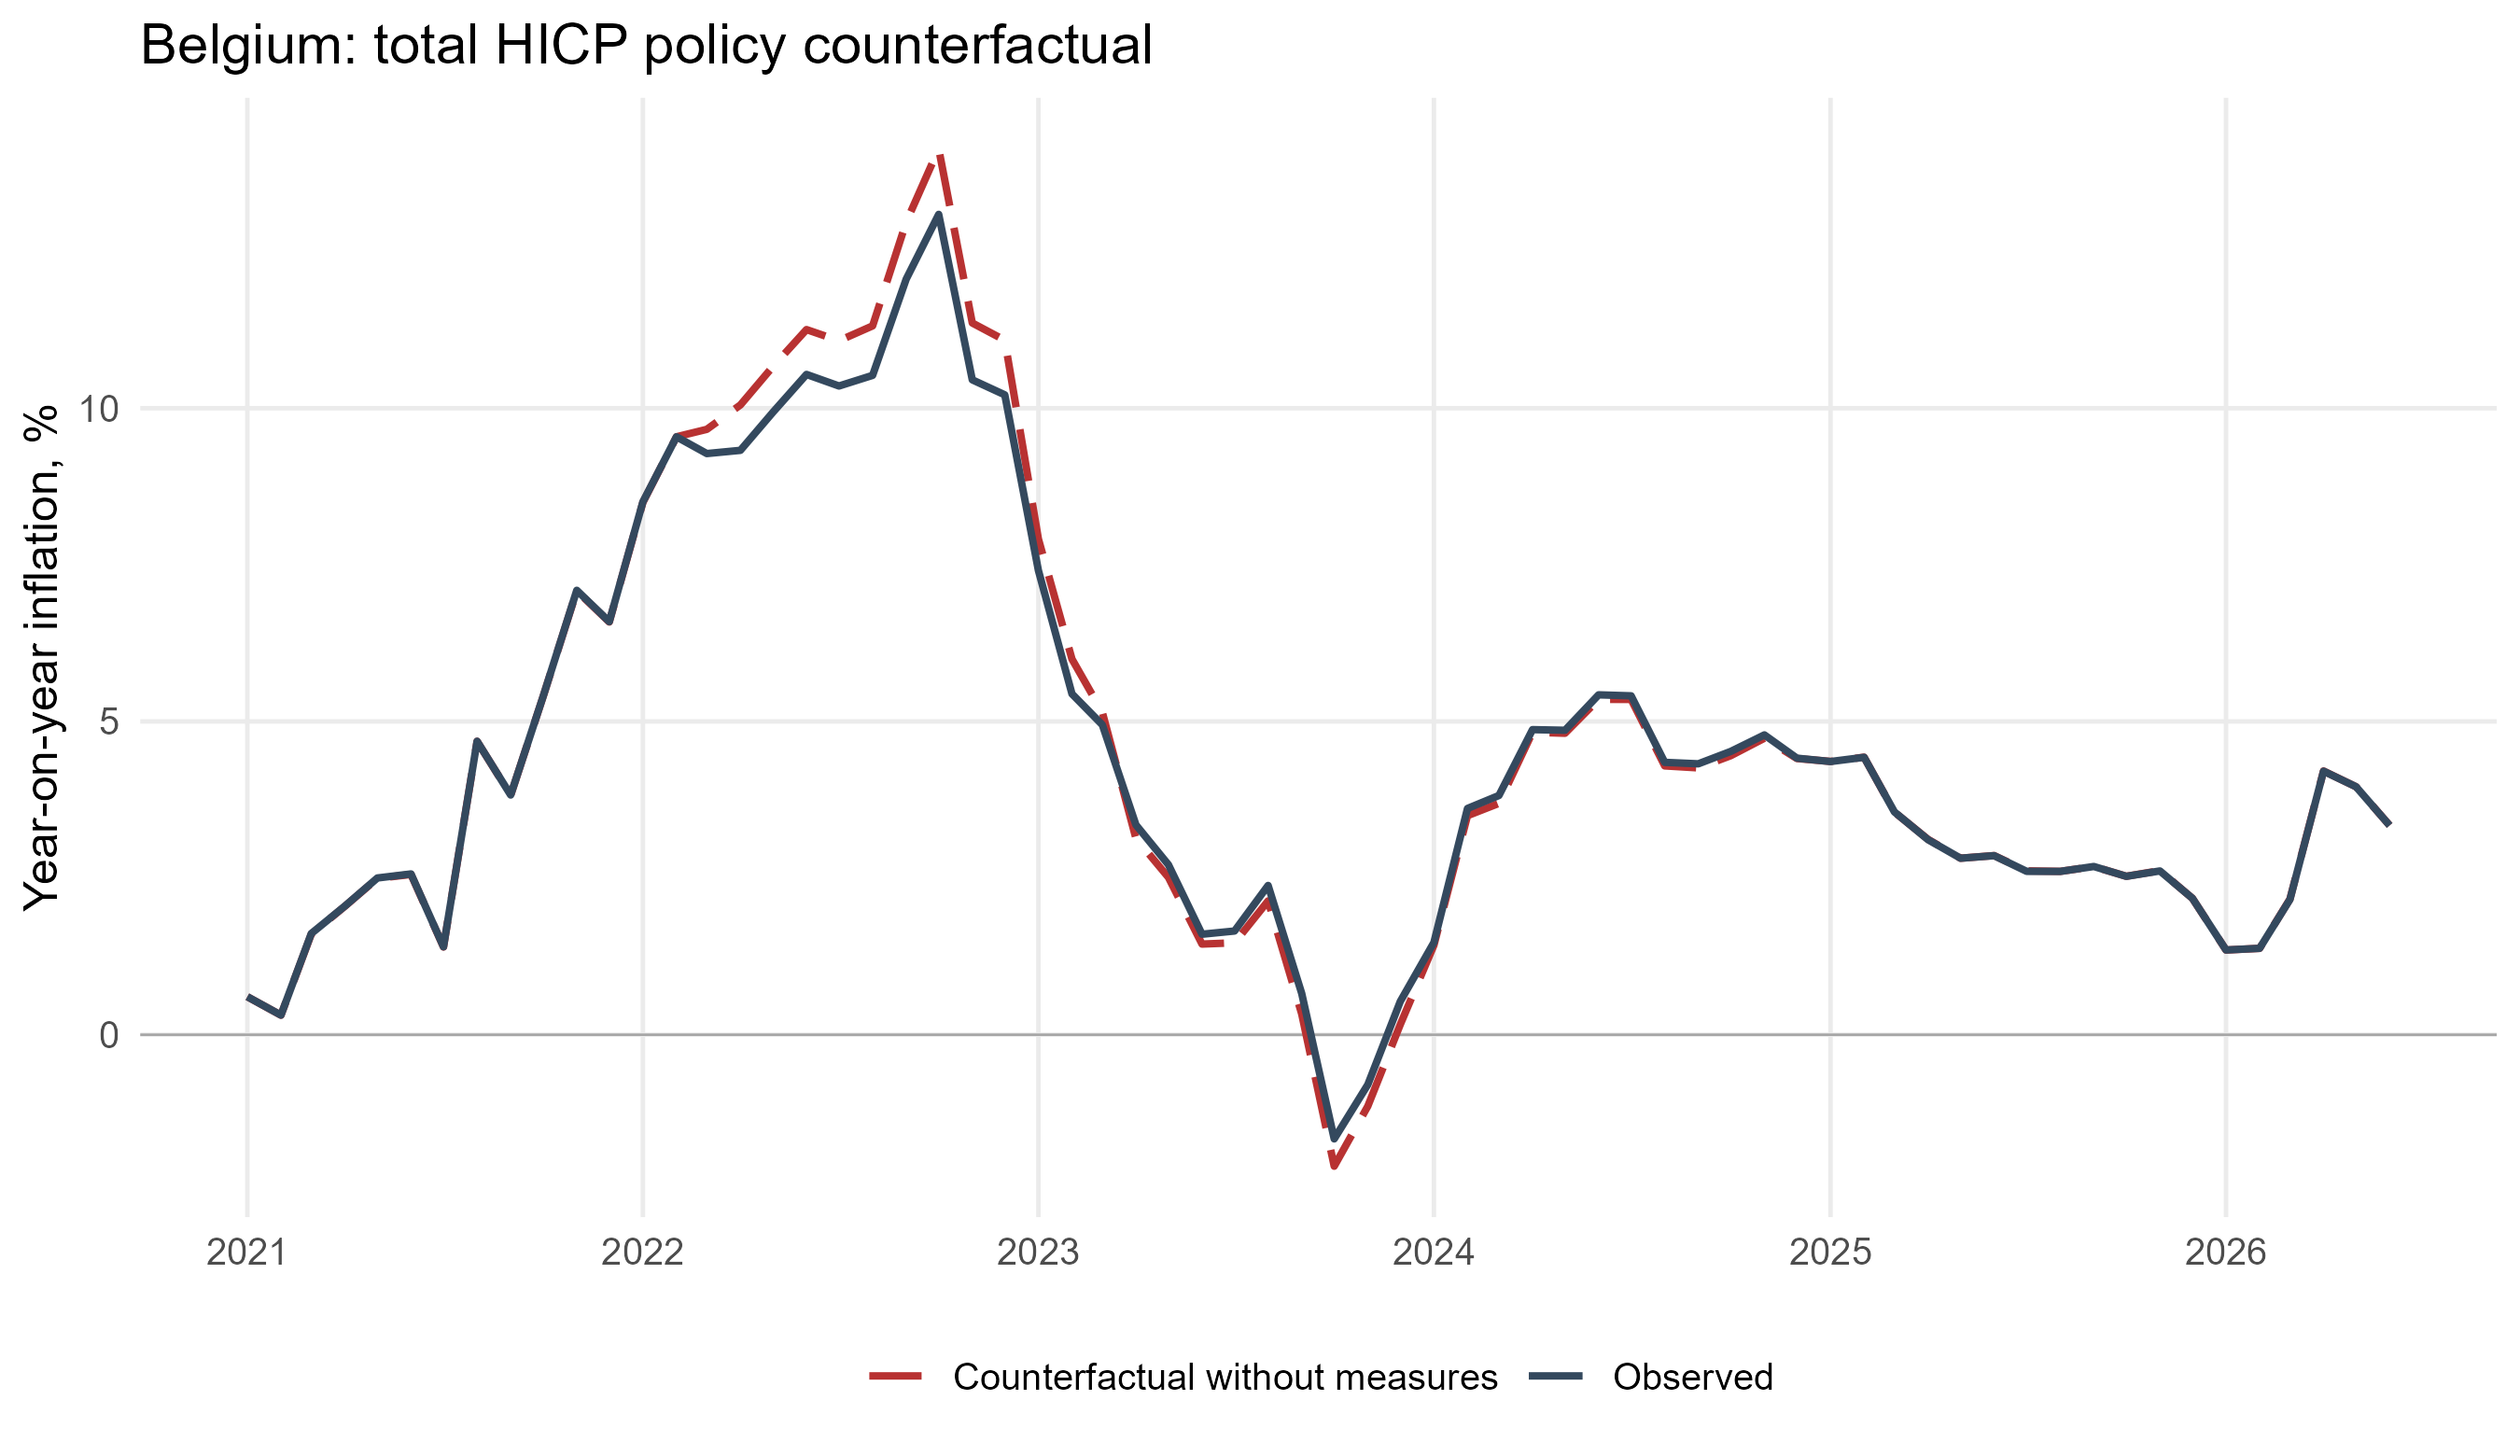
\includegraphics[width=0.86\textwidth,height=0.38\textheight,keepaspectratio]{fig/policy_total_cpi_counterfactual_inflation_BE_belgium.png}
\caption{Belgium: observed and counterfactual inflation}
\end{figure}

\subsection{Cyprus}
\begin{figure}[H]
\centering
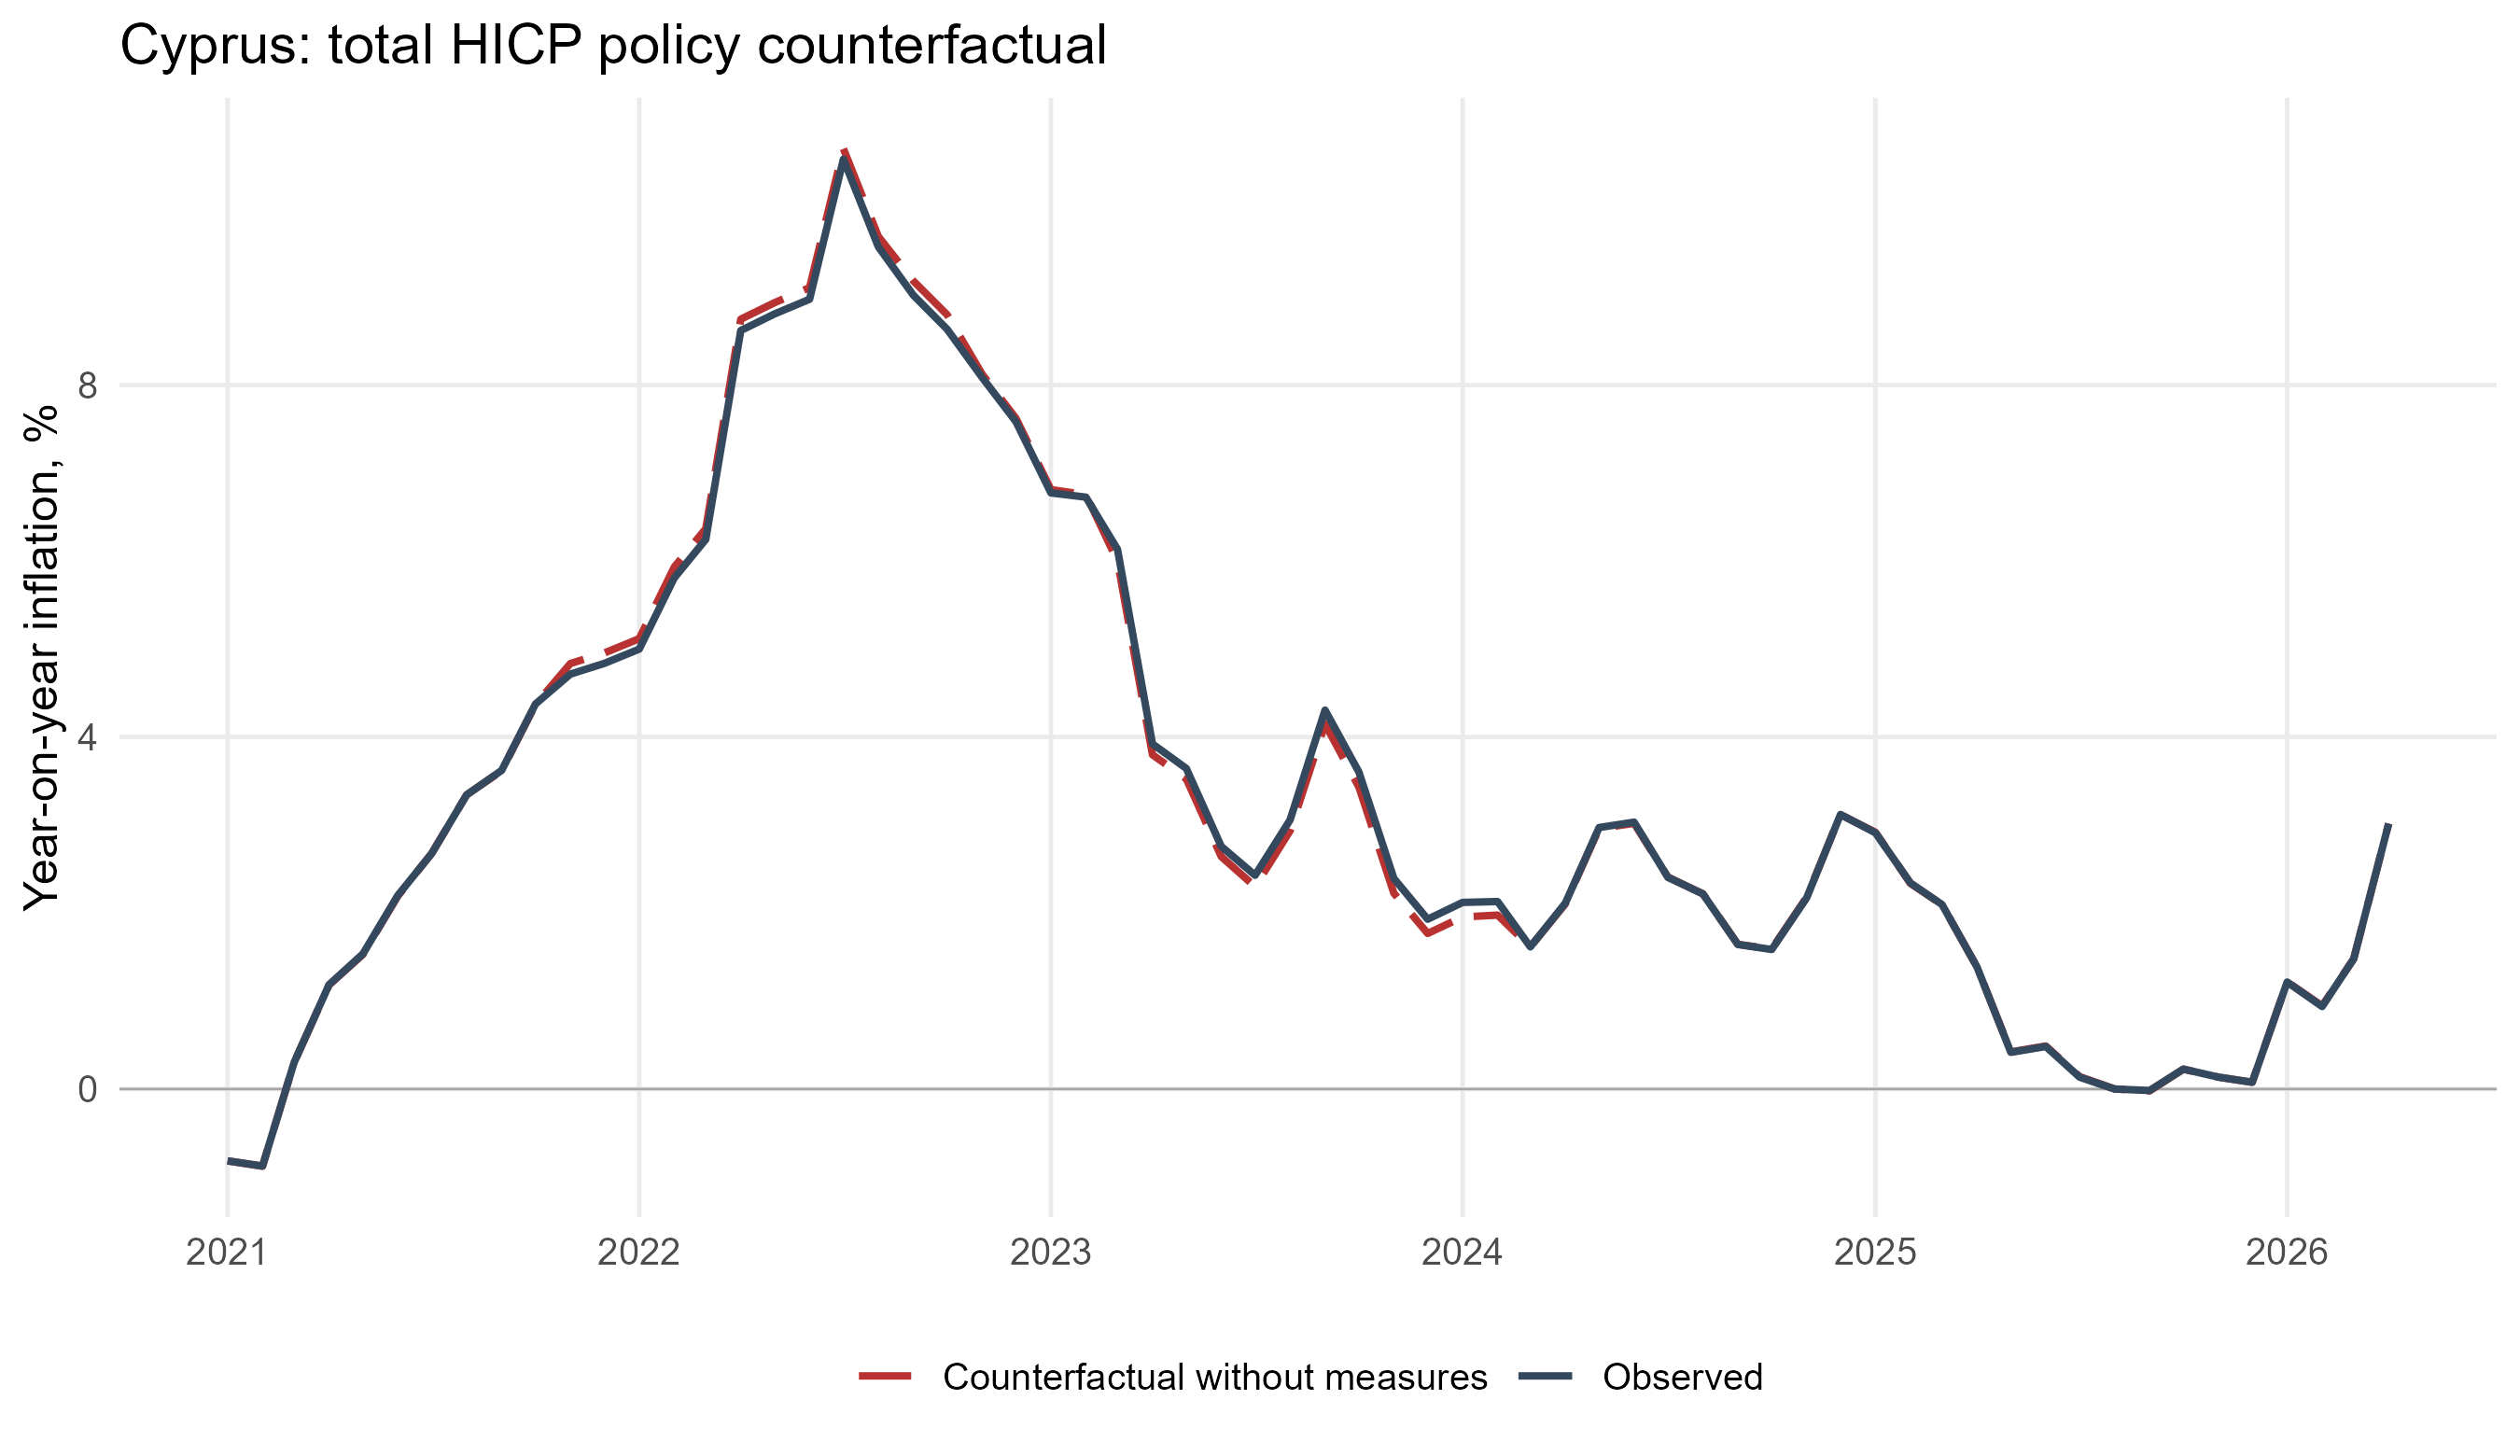
\includegraphics[width=0.86\textwidth,height=0.38\textheight,keepaspectratio]{fig/policy_total_cpi_counterfactual_inflation_CY_cyprus.png}
\caption{Cyprus: observed and counterfactual inflation}
\end{figure}

\subsection{Germany}
\begin{figure}[H]
\centering
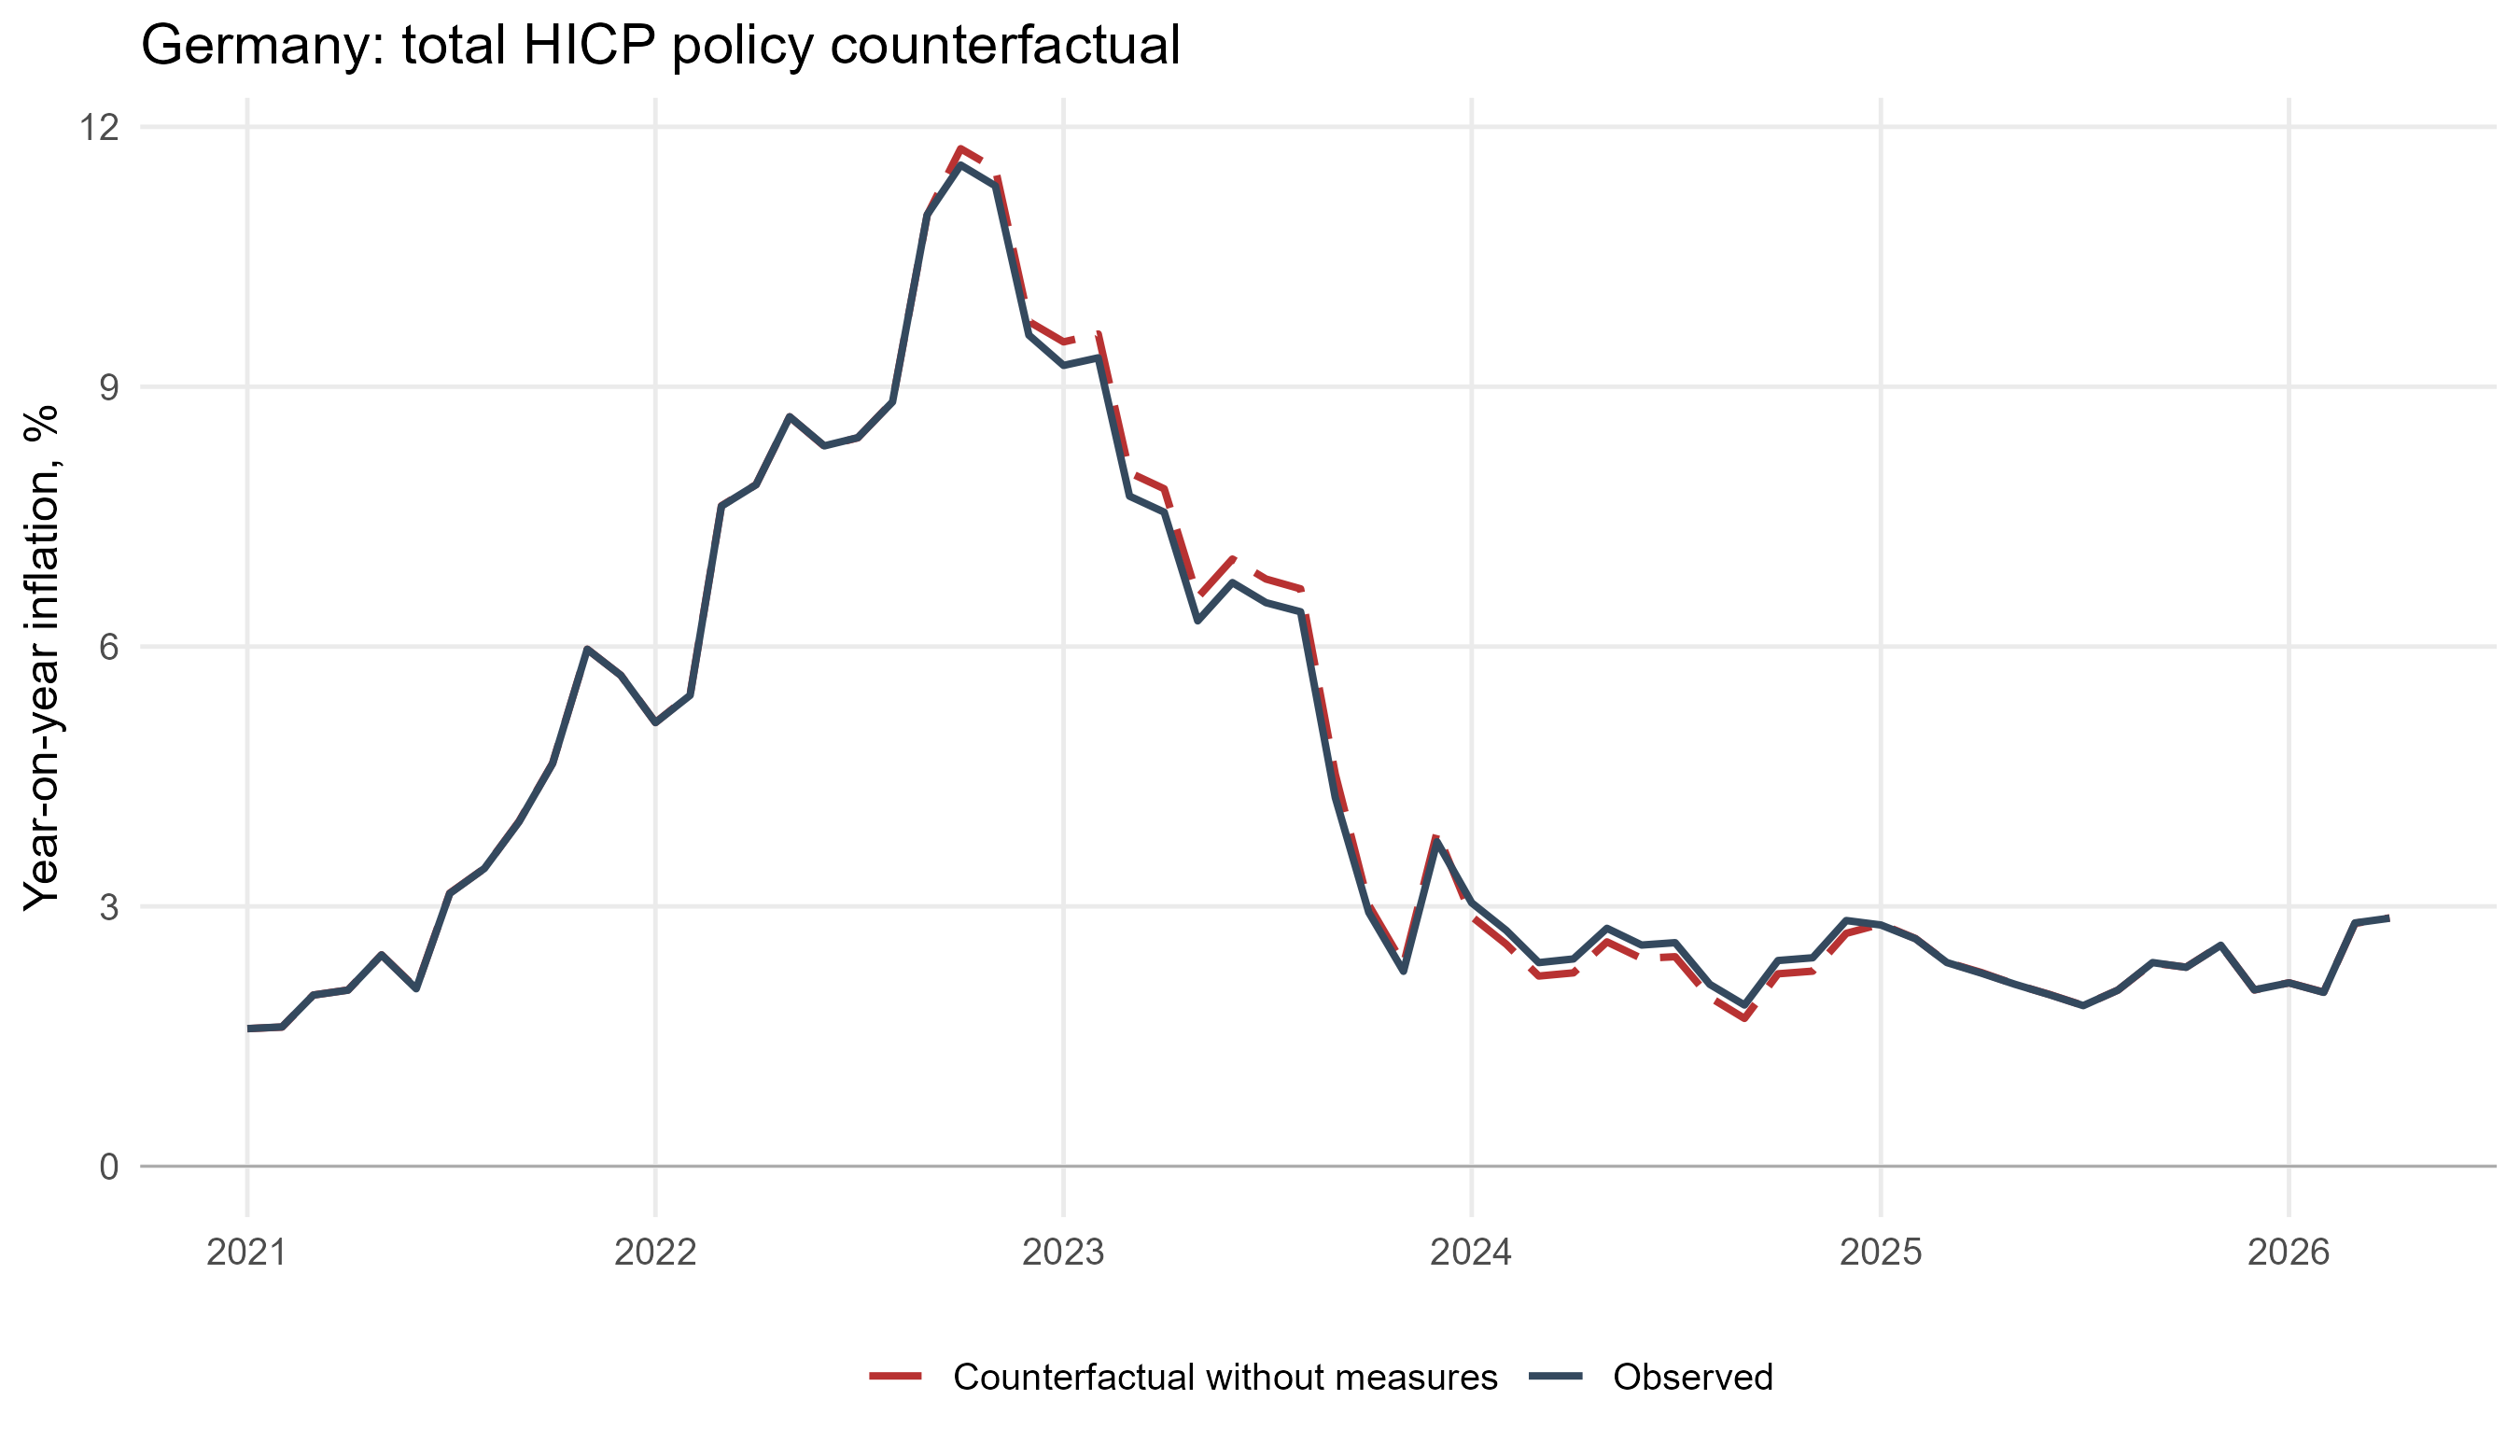
\includegraphics[width=0.86\textwidth,height=0.38\textheight,keepaspectratio]{fig/policy_total_cpi_counterfactual_inflation_DE_germany.png}
\caption{Germany: observed and counterfactual inflation}
\end{figure}

\subsection{Greece}
\begin{figure}[H]
\centering
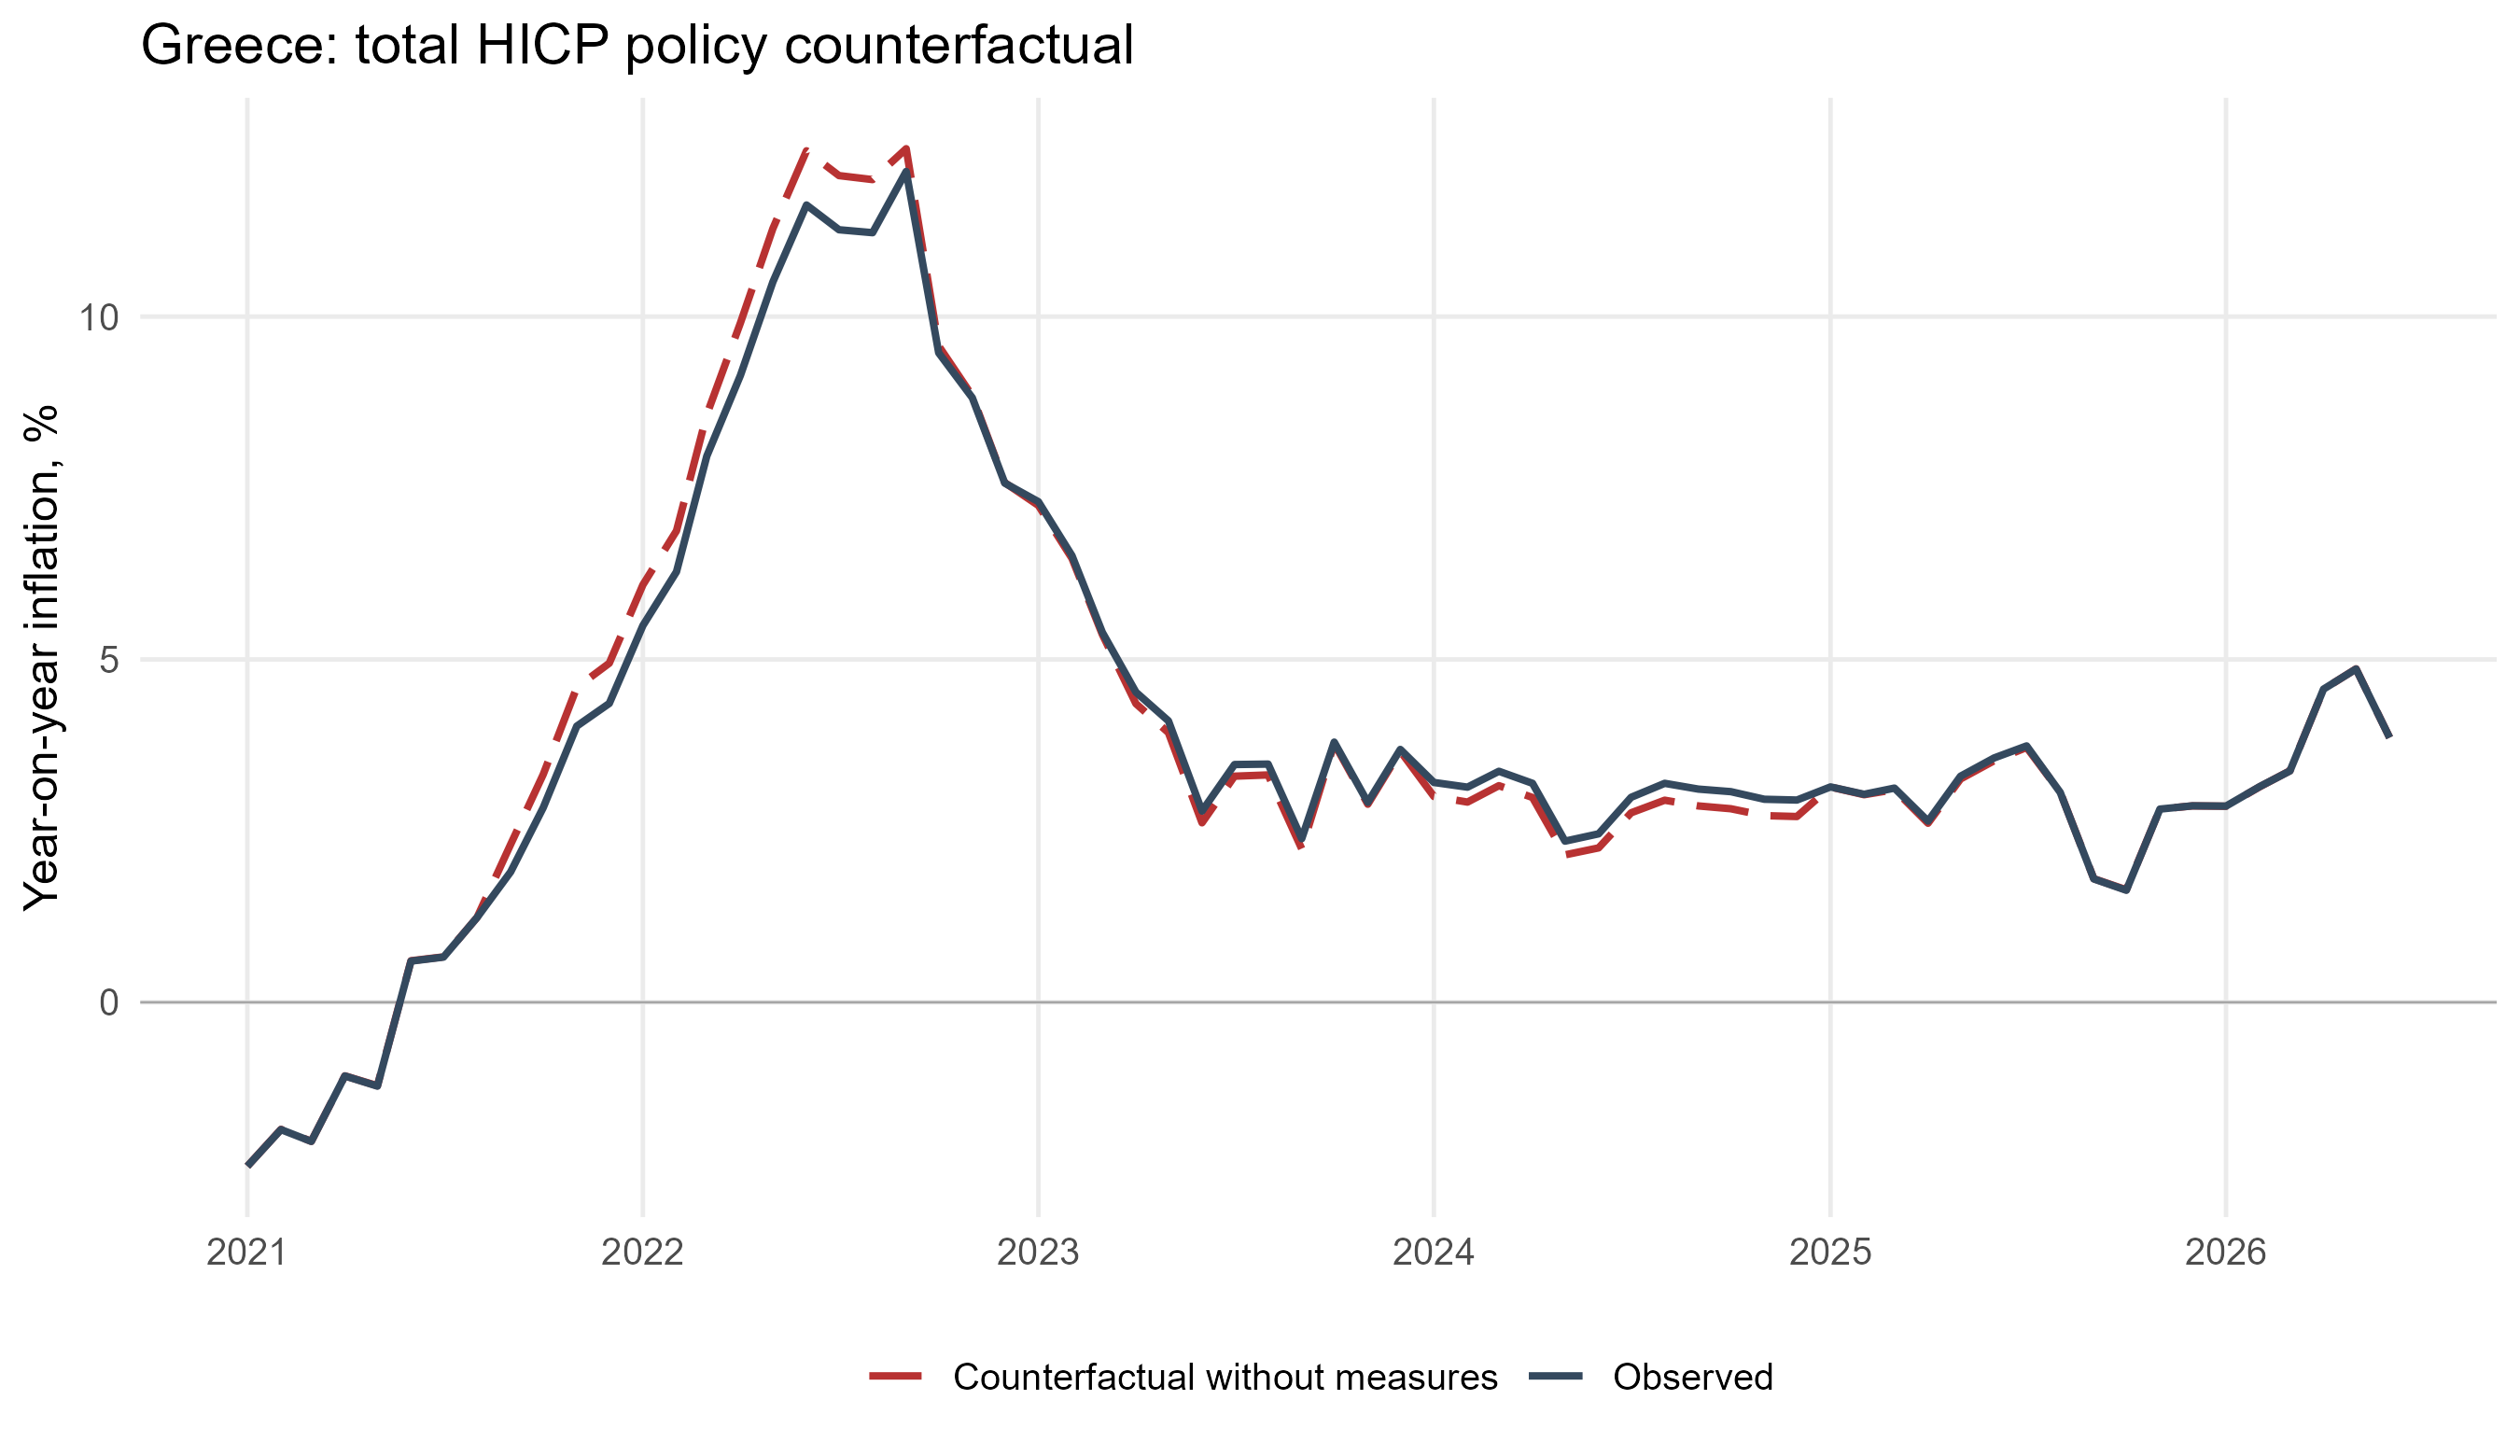
\includegraphics[width=0.86\textwidth,height=0.38\textheight,keepaspectratio]{fig/policy_total_cpi_counterfactual_inflation_EL_greece.png}
\caption{Greece: observed and counterfactual inflation}
\end{figure}

\subsection{Spain}
\begin{figure}[H]
\centering
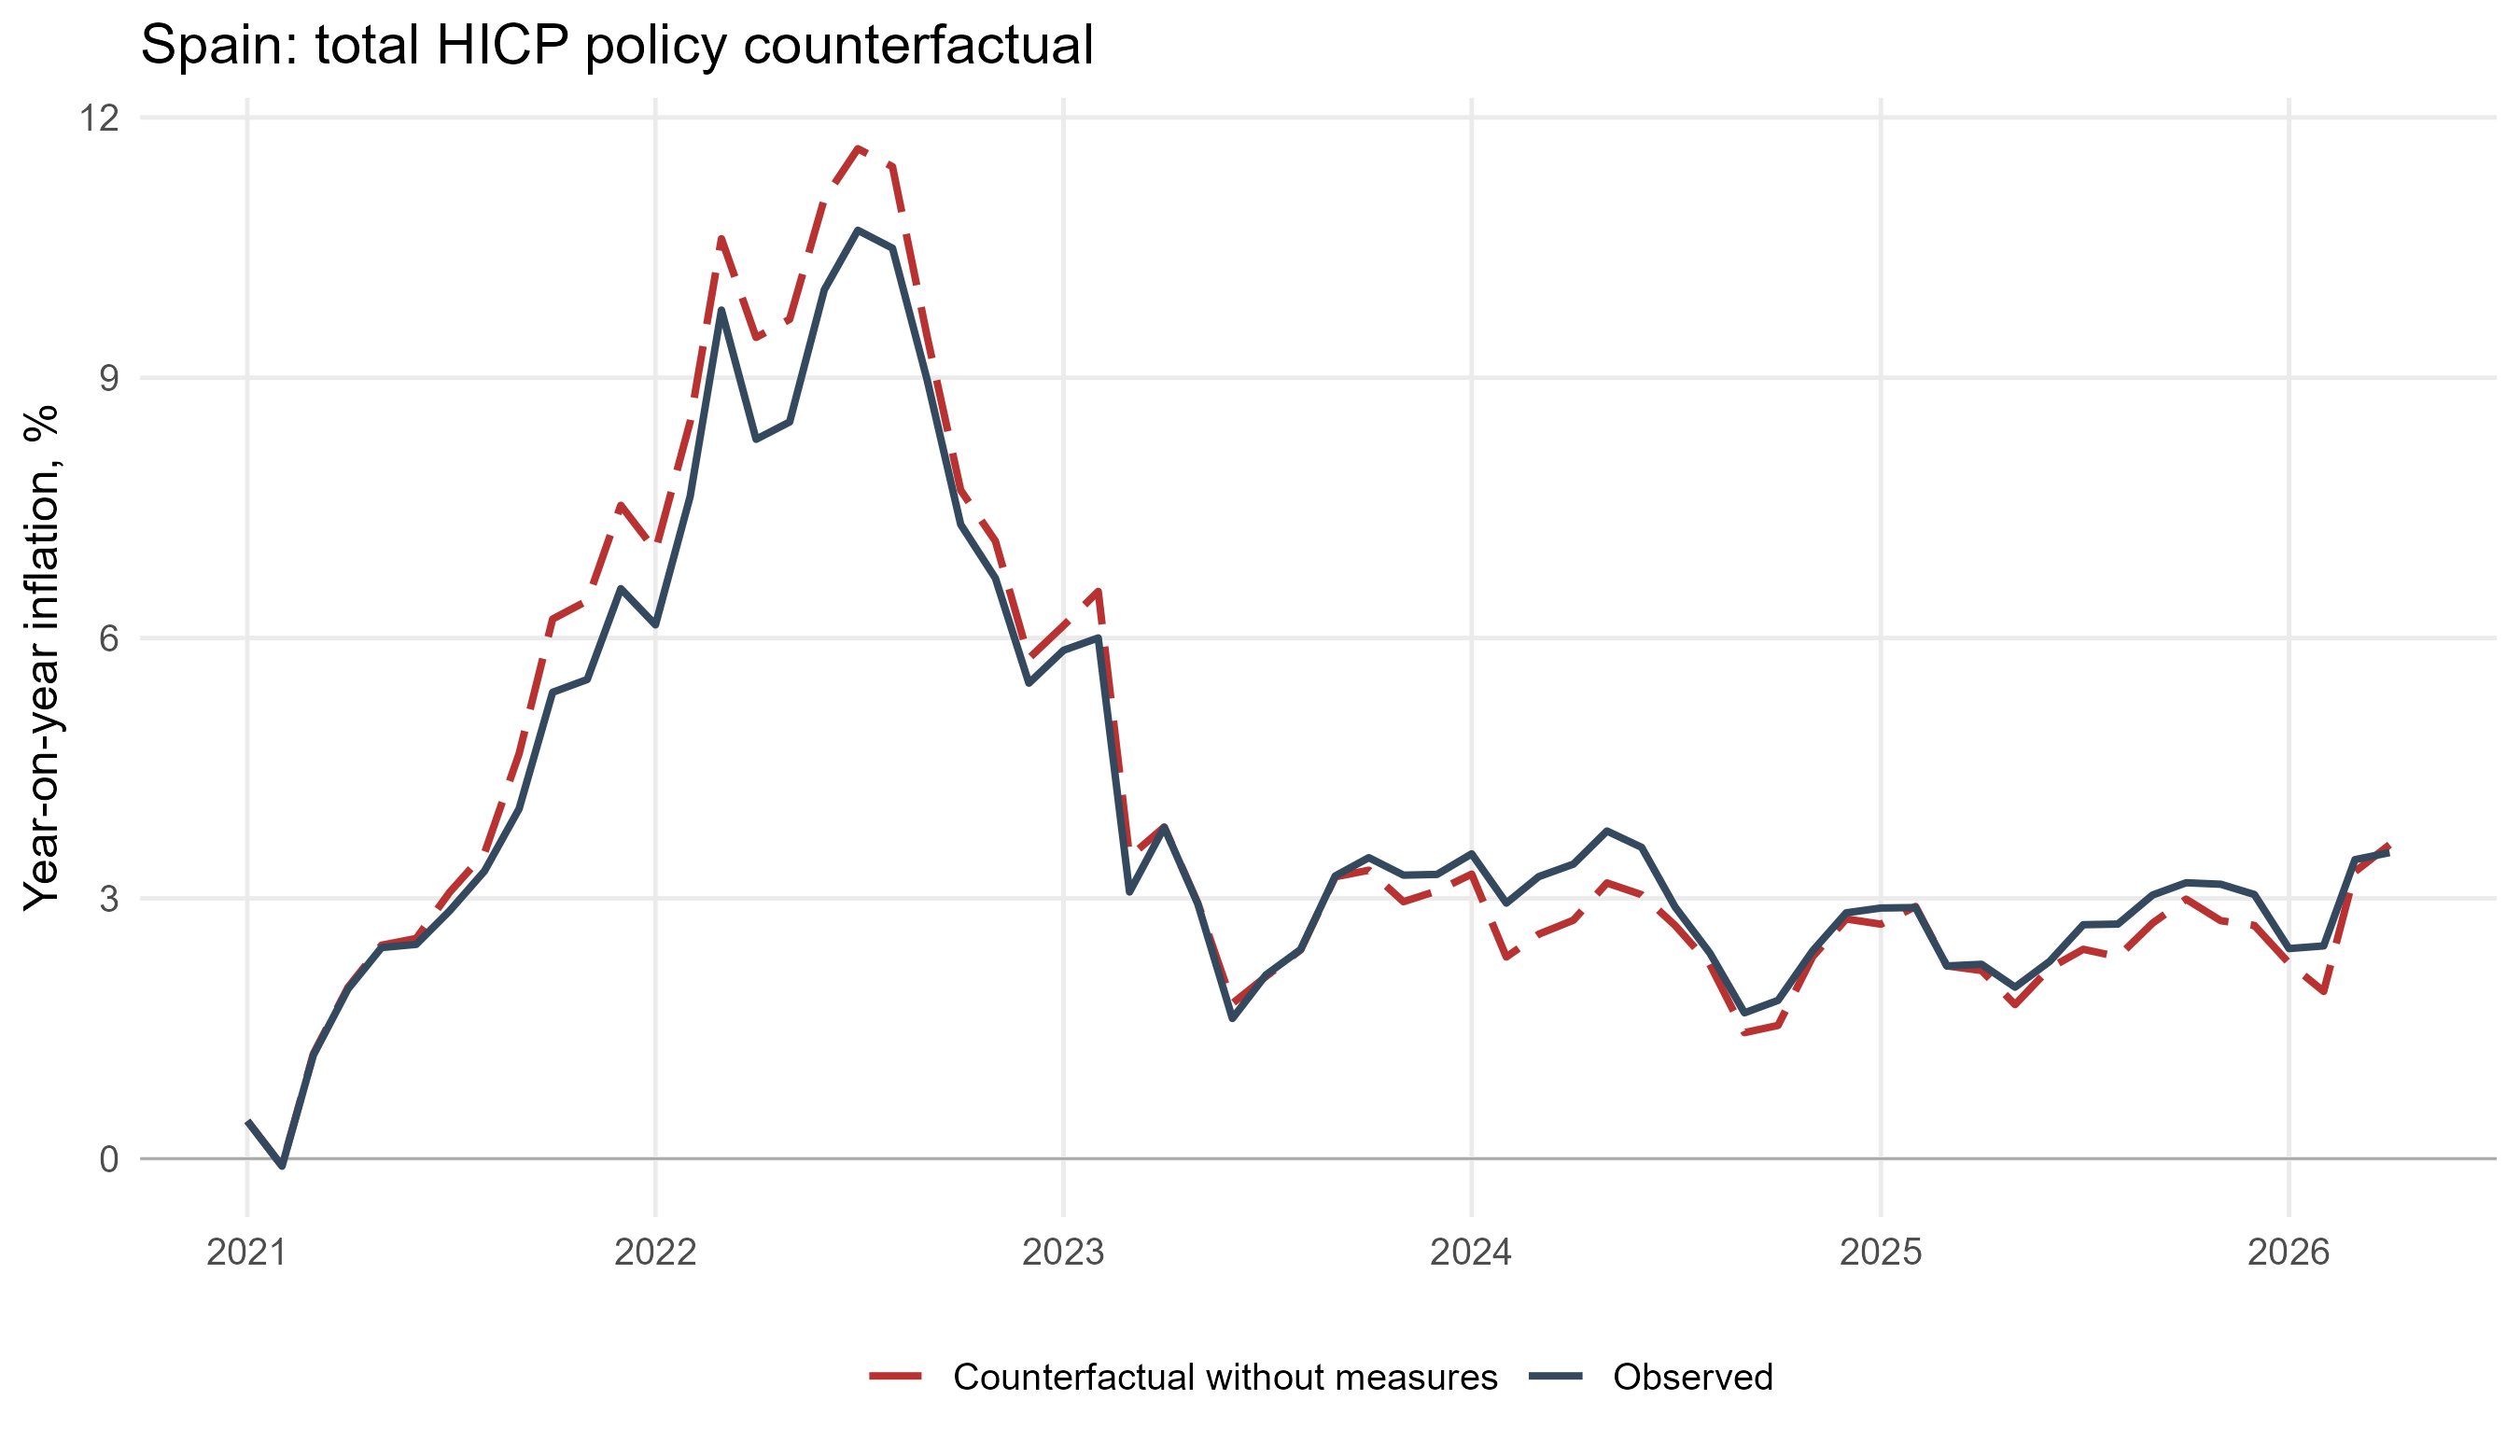
\includegraphics[width=0.86\textwidth,height=0.38\textheight,keepaspectratio]{fig/policy_total_cpi_counterfactual_inflation_ES_spain.png}
\caption{Spain: observed and counterfactual inflation}
\end{figure}

\subsection{Finland}
\begin{figure}[H]
\centering
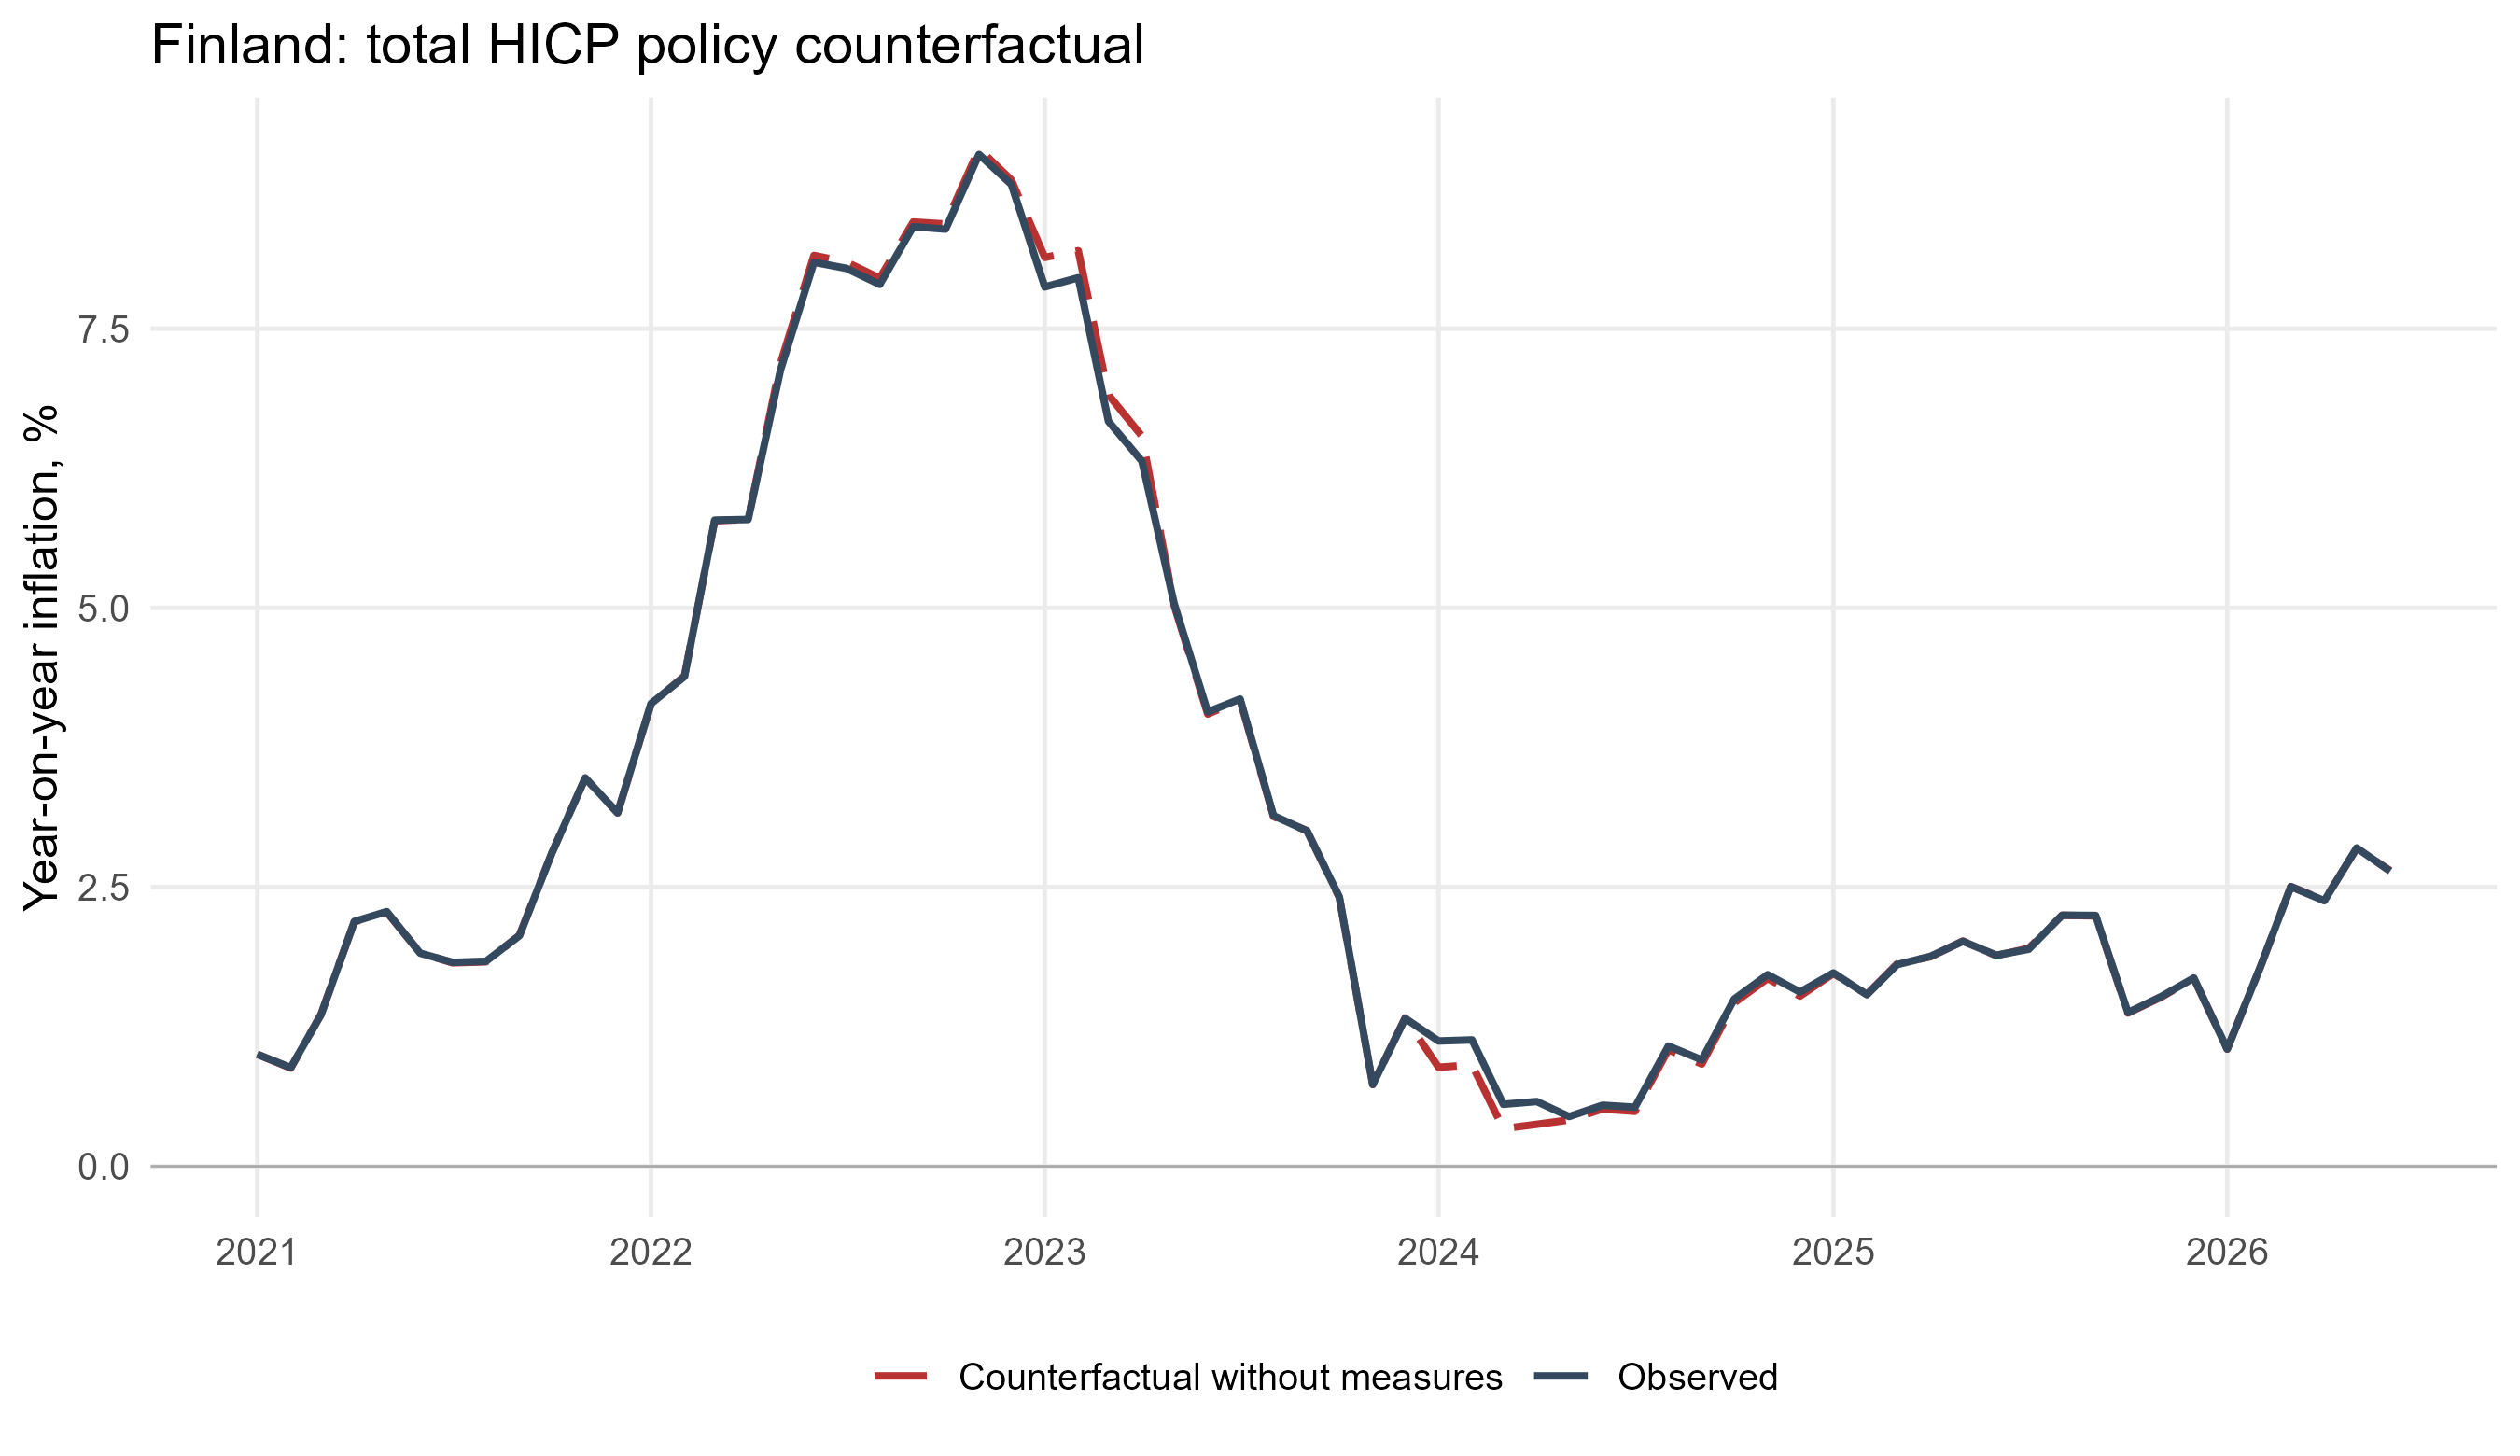
\includegraphics[width=0.86\textwidth,height=0.38\textheight,keepaspectratio]{fig/policy_total_cpi_counterfactual_inflation_FI_finland.png}
\caption{Finland: observed and counterfactual inflation}
\end{figure}

\subsection{France}
\begin{figure}[H]
\centering
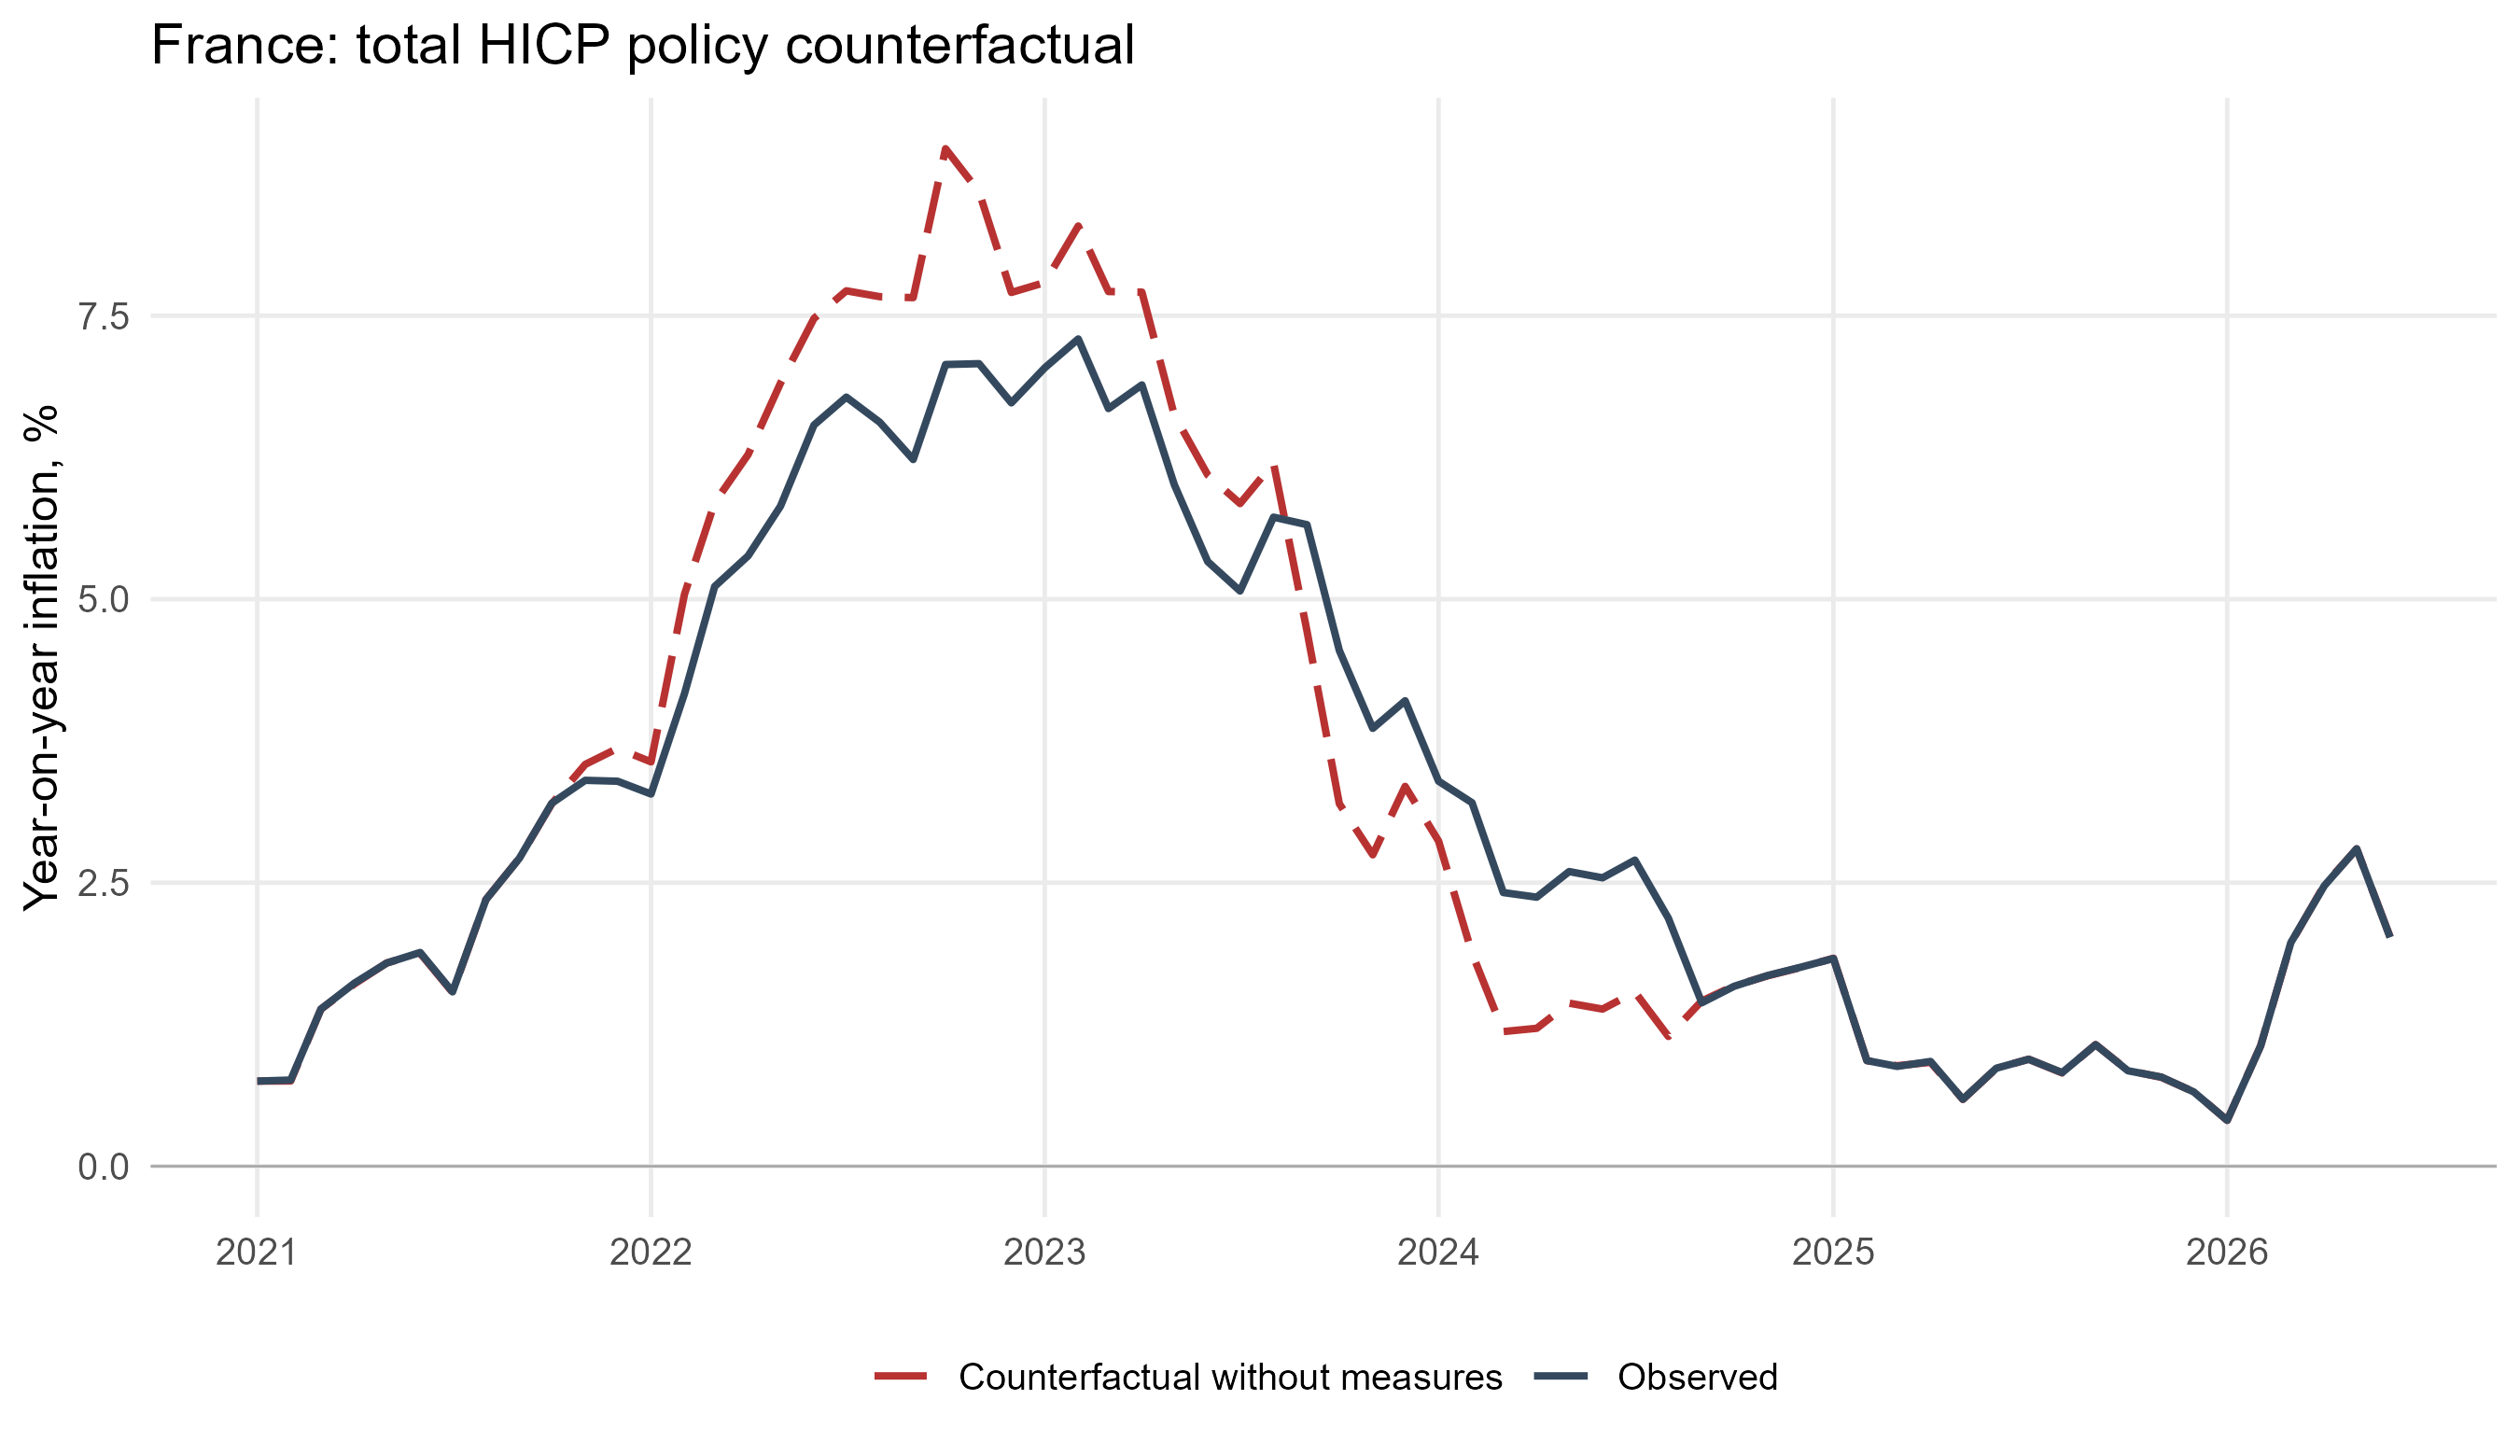
\includegraphics[width=0.86\textwidth,height=0.38\textheight,keepaspectratio]{fig/policy_total_cpi_counterfactual_inflation_FR_france.png}
\caption{France: observed and counterfactual inflation}
\end{figure}

\subsection{Croatia}
\begin{figure}[H]
\centering
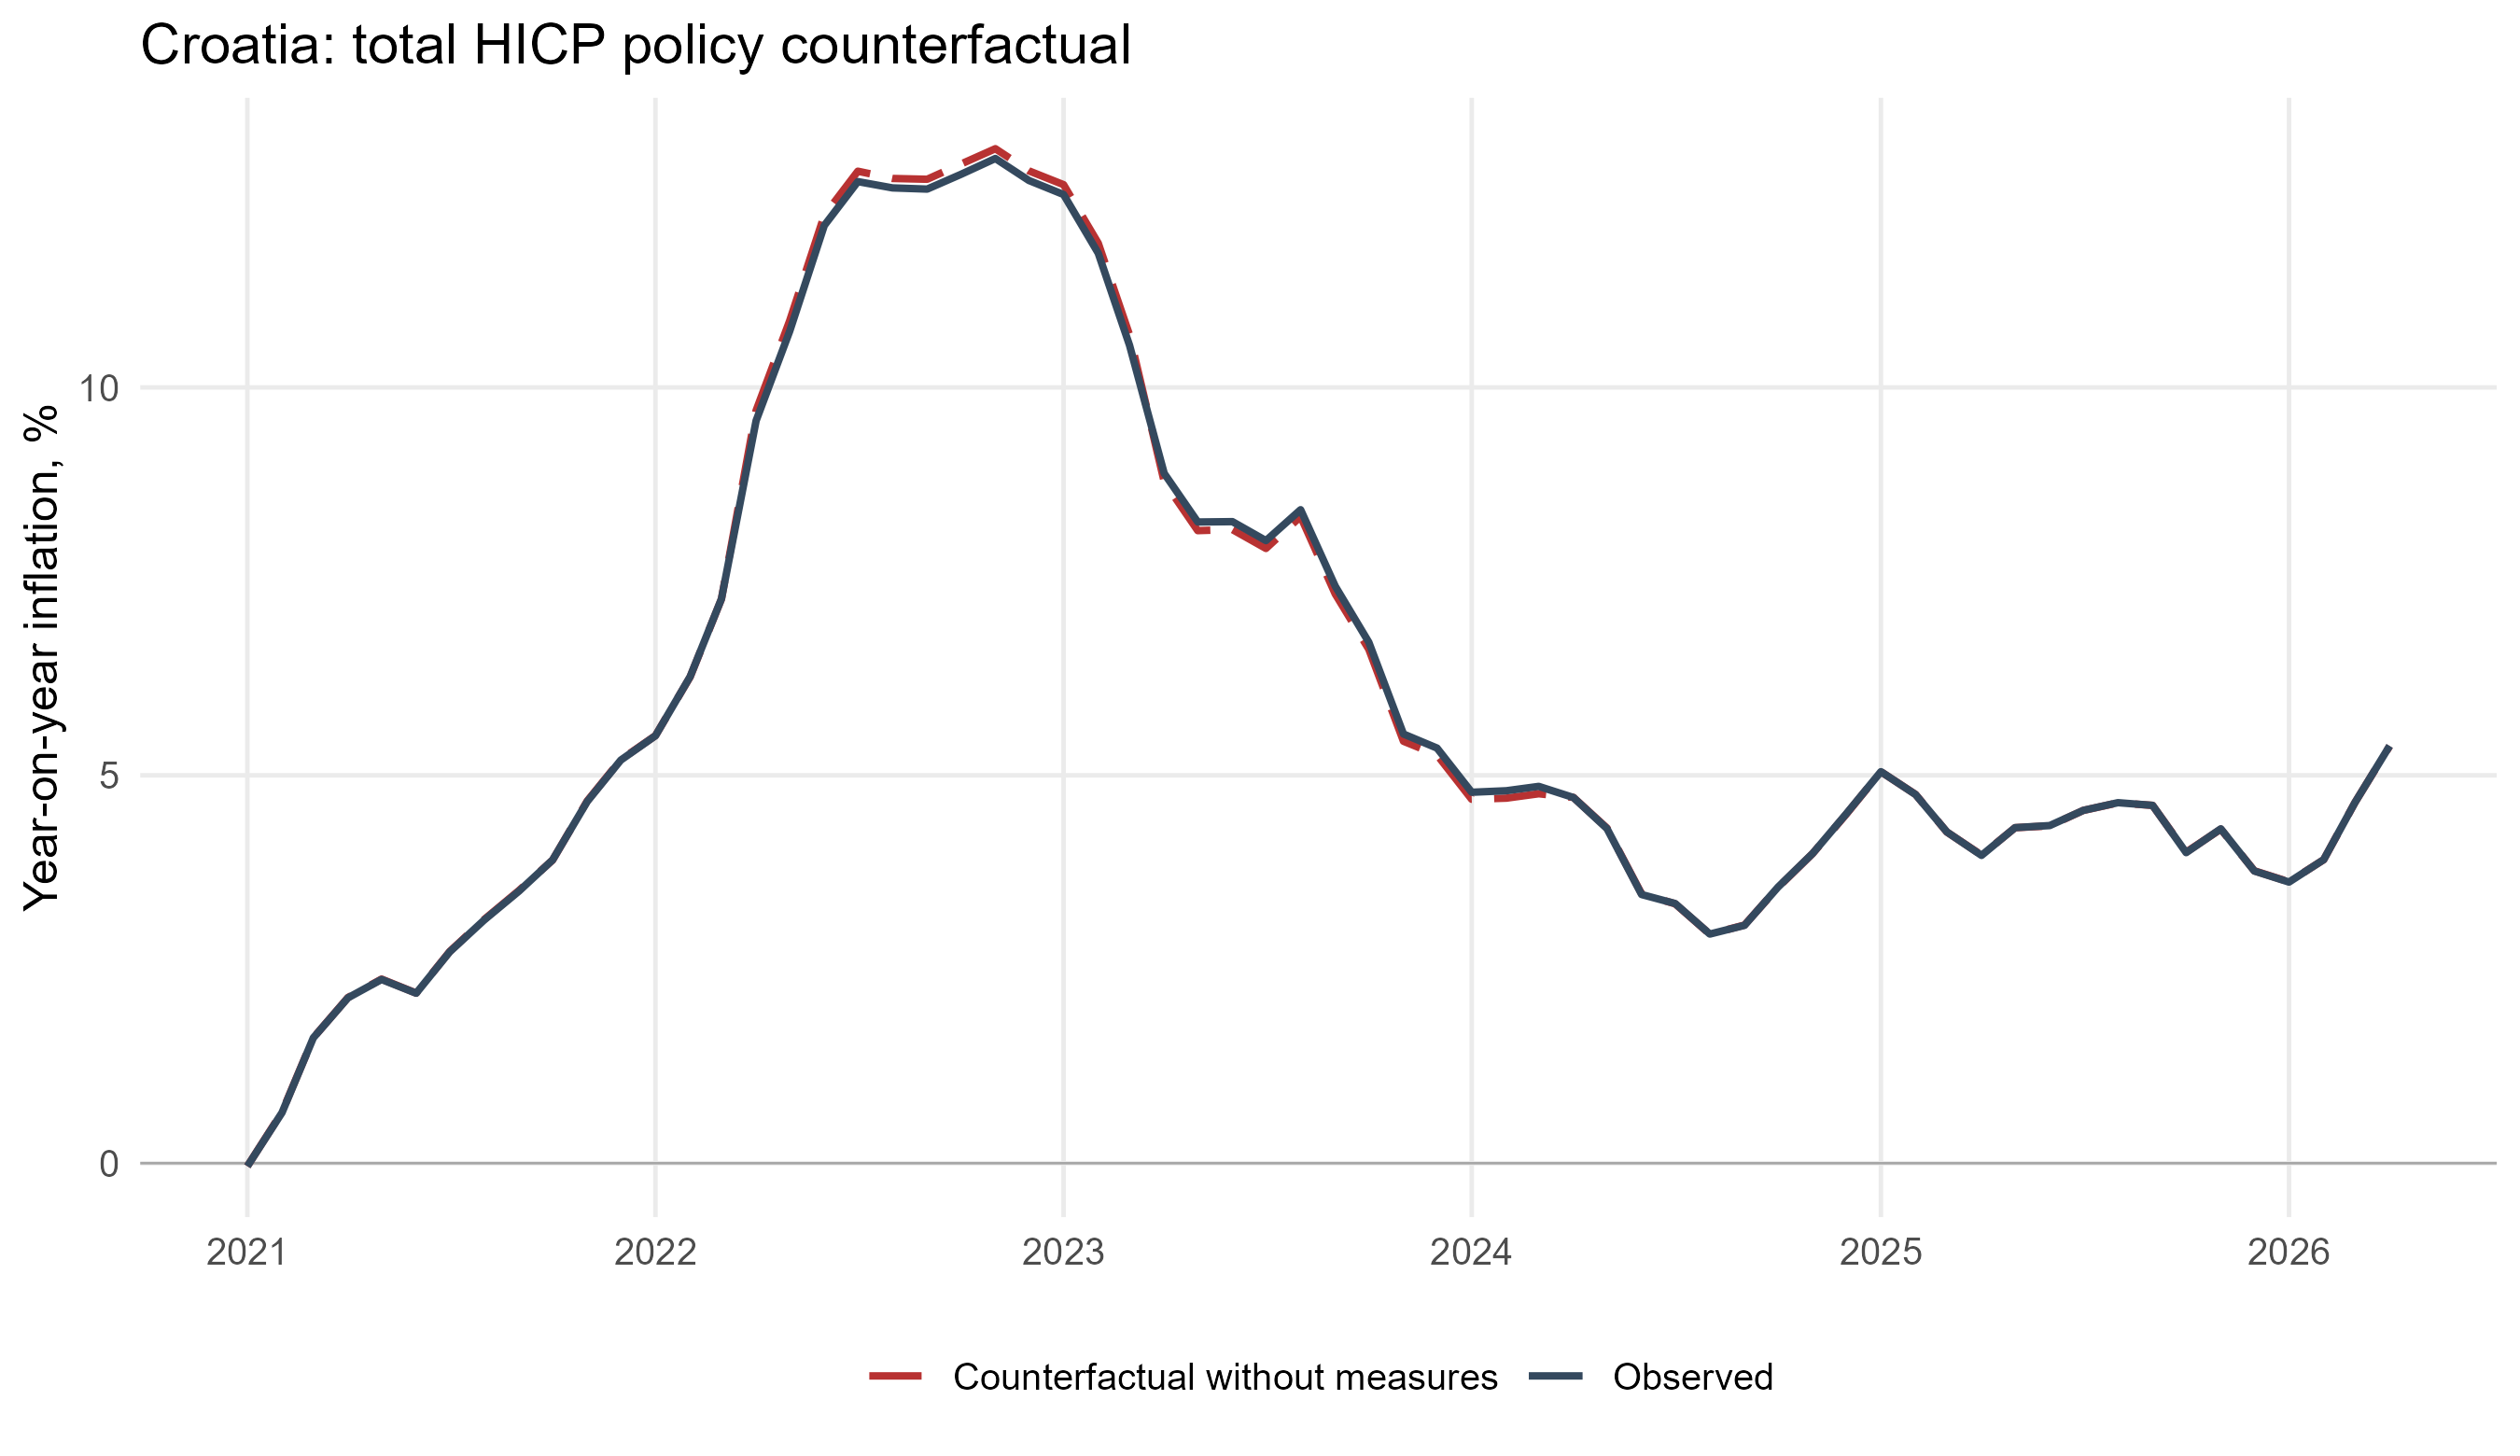
\includegraphics[width=0.86\textwidth,height=0.38\textheight,keepaspectratio]{fig/policy_total_cpi_counterfactual_inflation_HR_croatia.png}
\caption{Croatia: observed and counterfactual inflation}
\end{figure}

\subsection{Ireland}
\begin{figure}[H]
\centering
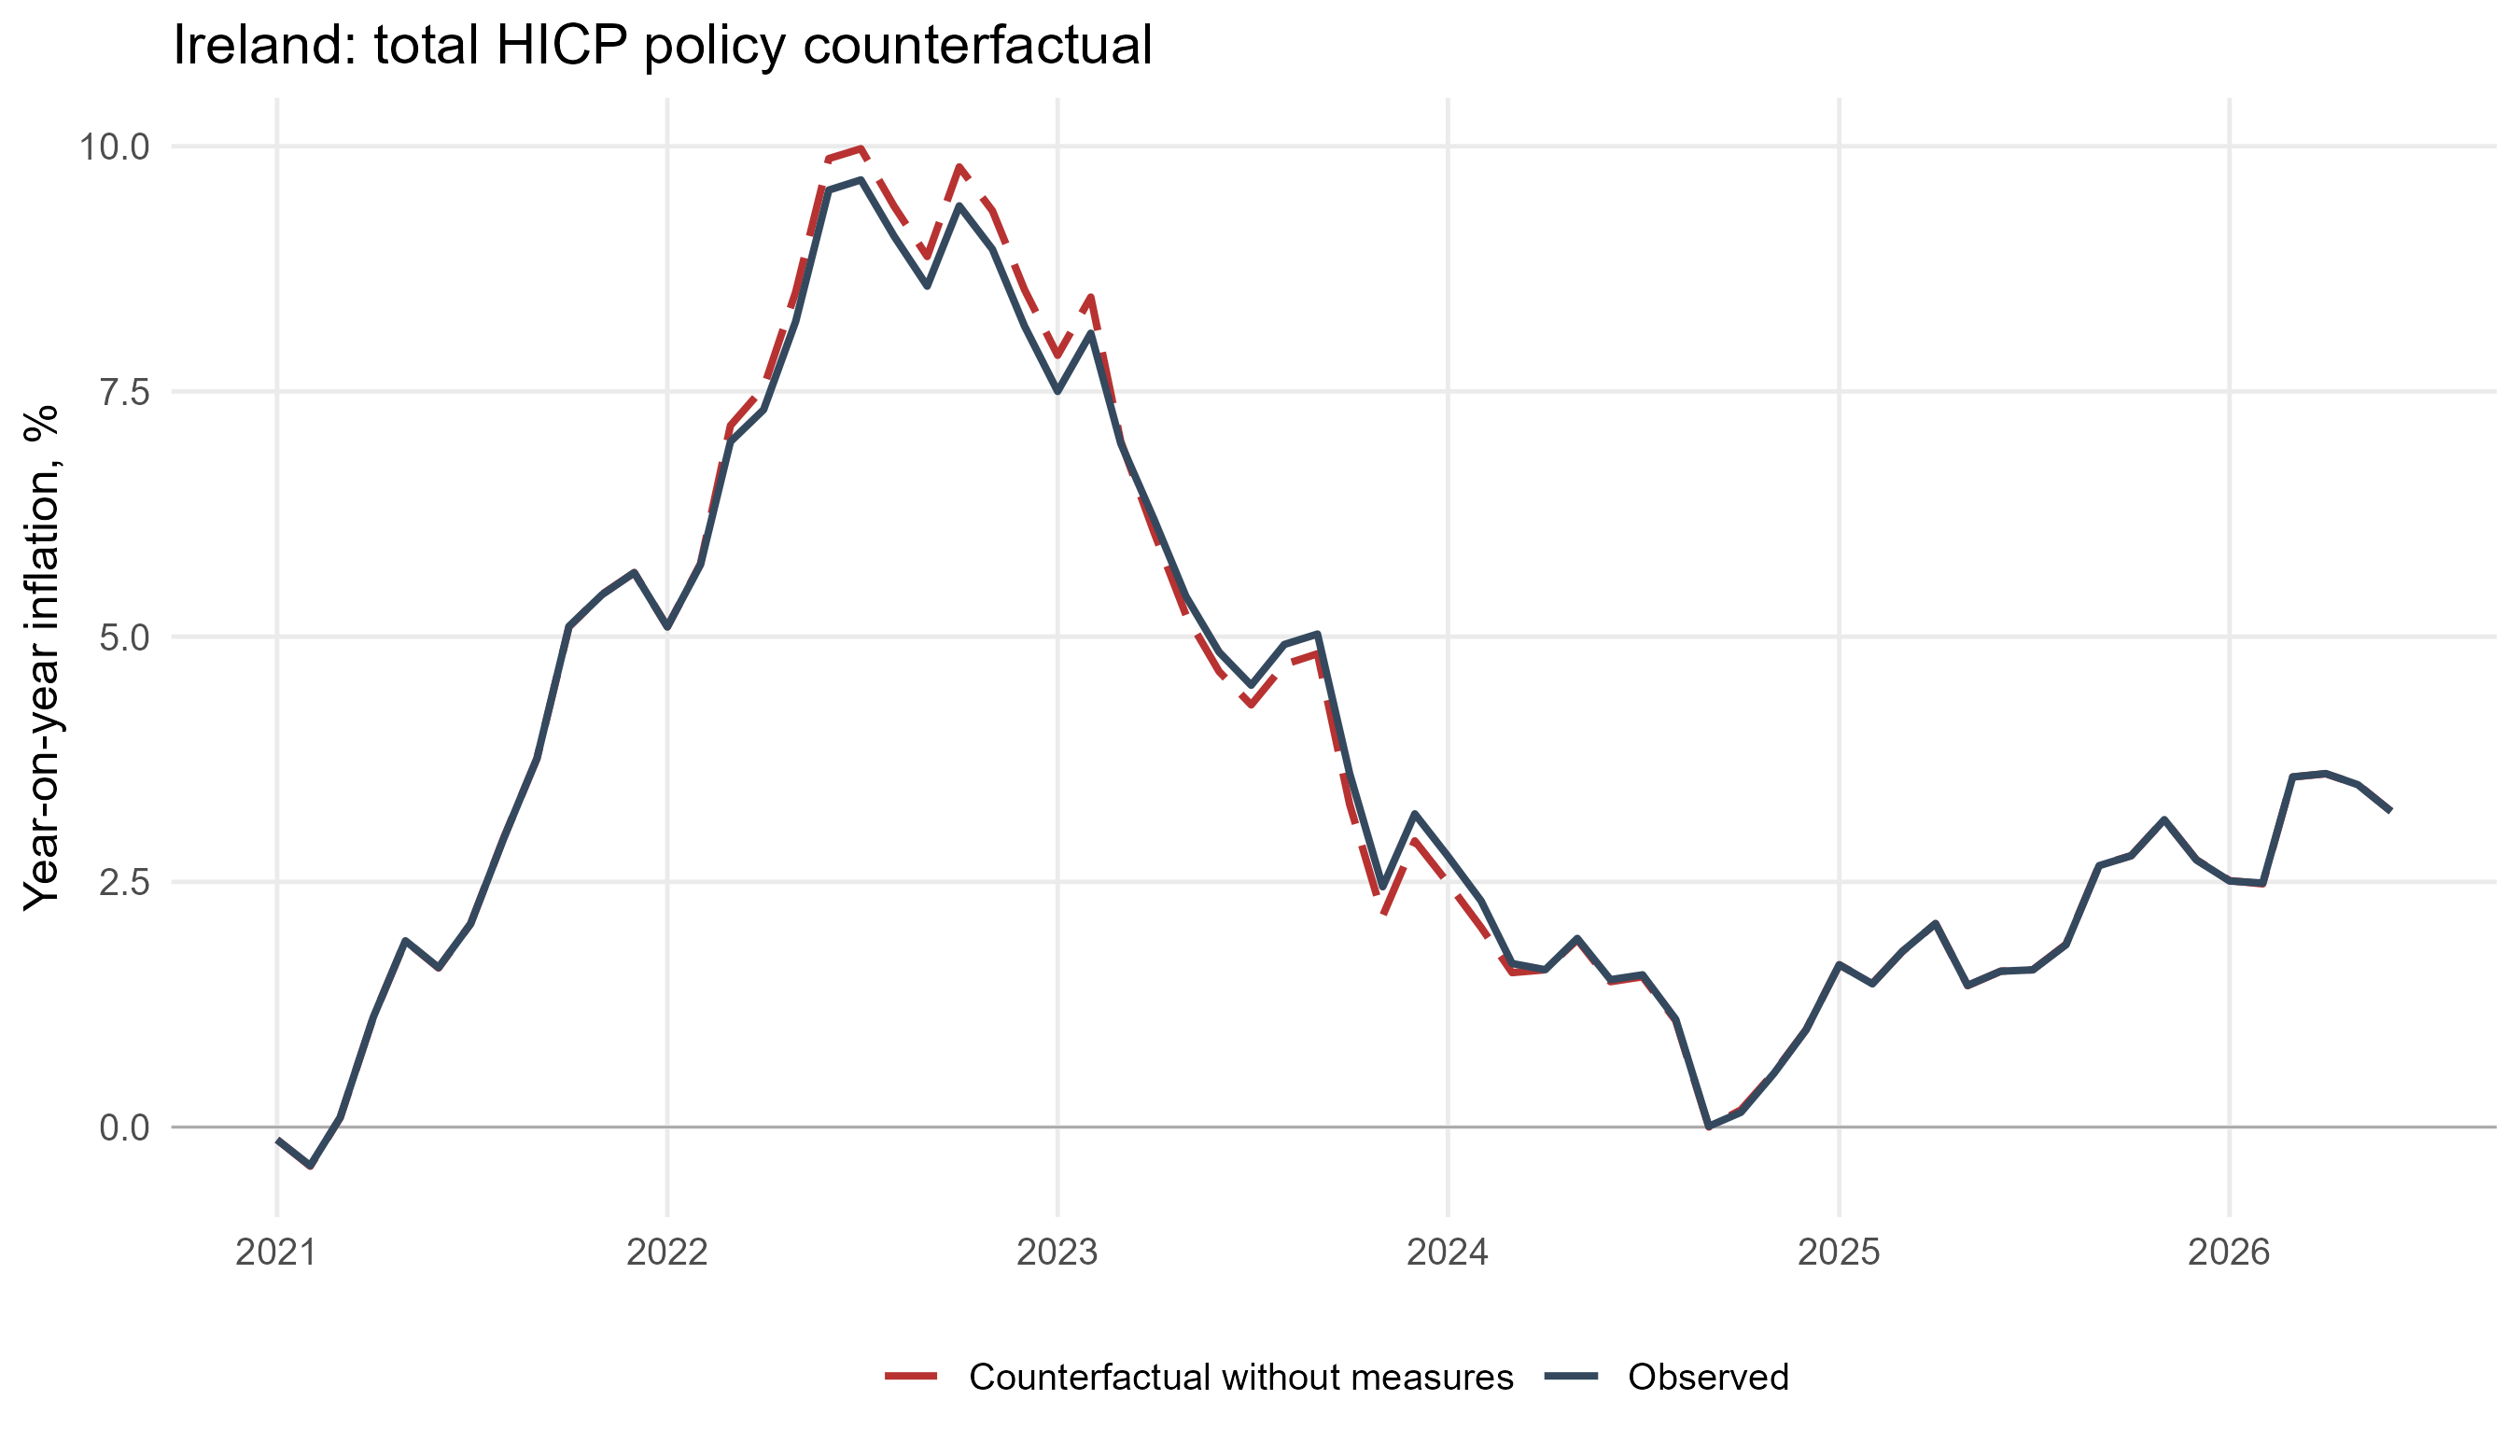
\includegraphics[width=0.86\textwidth,height=0.38\textheight,keepaspectratio]{fig/policy_total_cpi_counterfactual_inflation_IE_ireland.png}
\caption{Ireland: observed and counterfactual inflation}
\end{figure}

\subsection{Italy}
\begin{figure}[H]
\centering
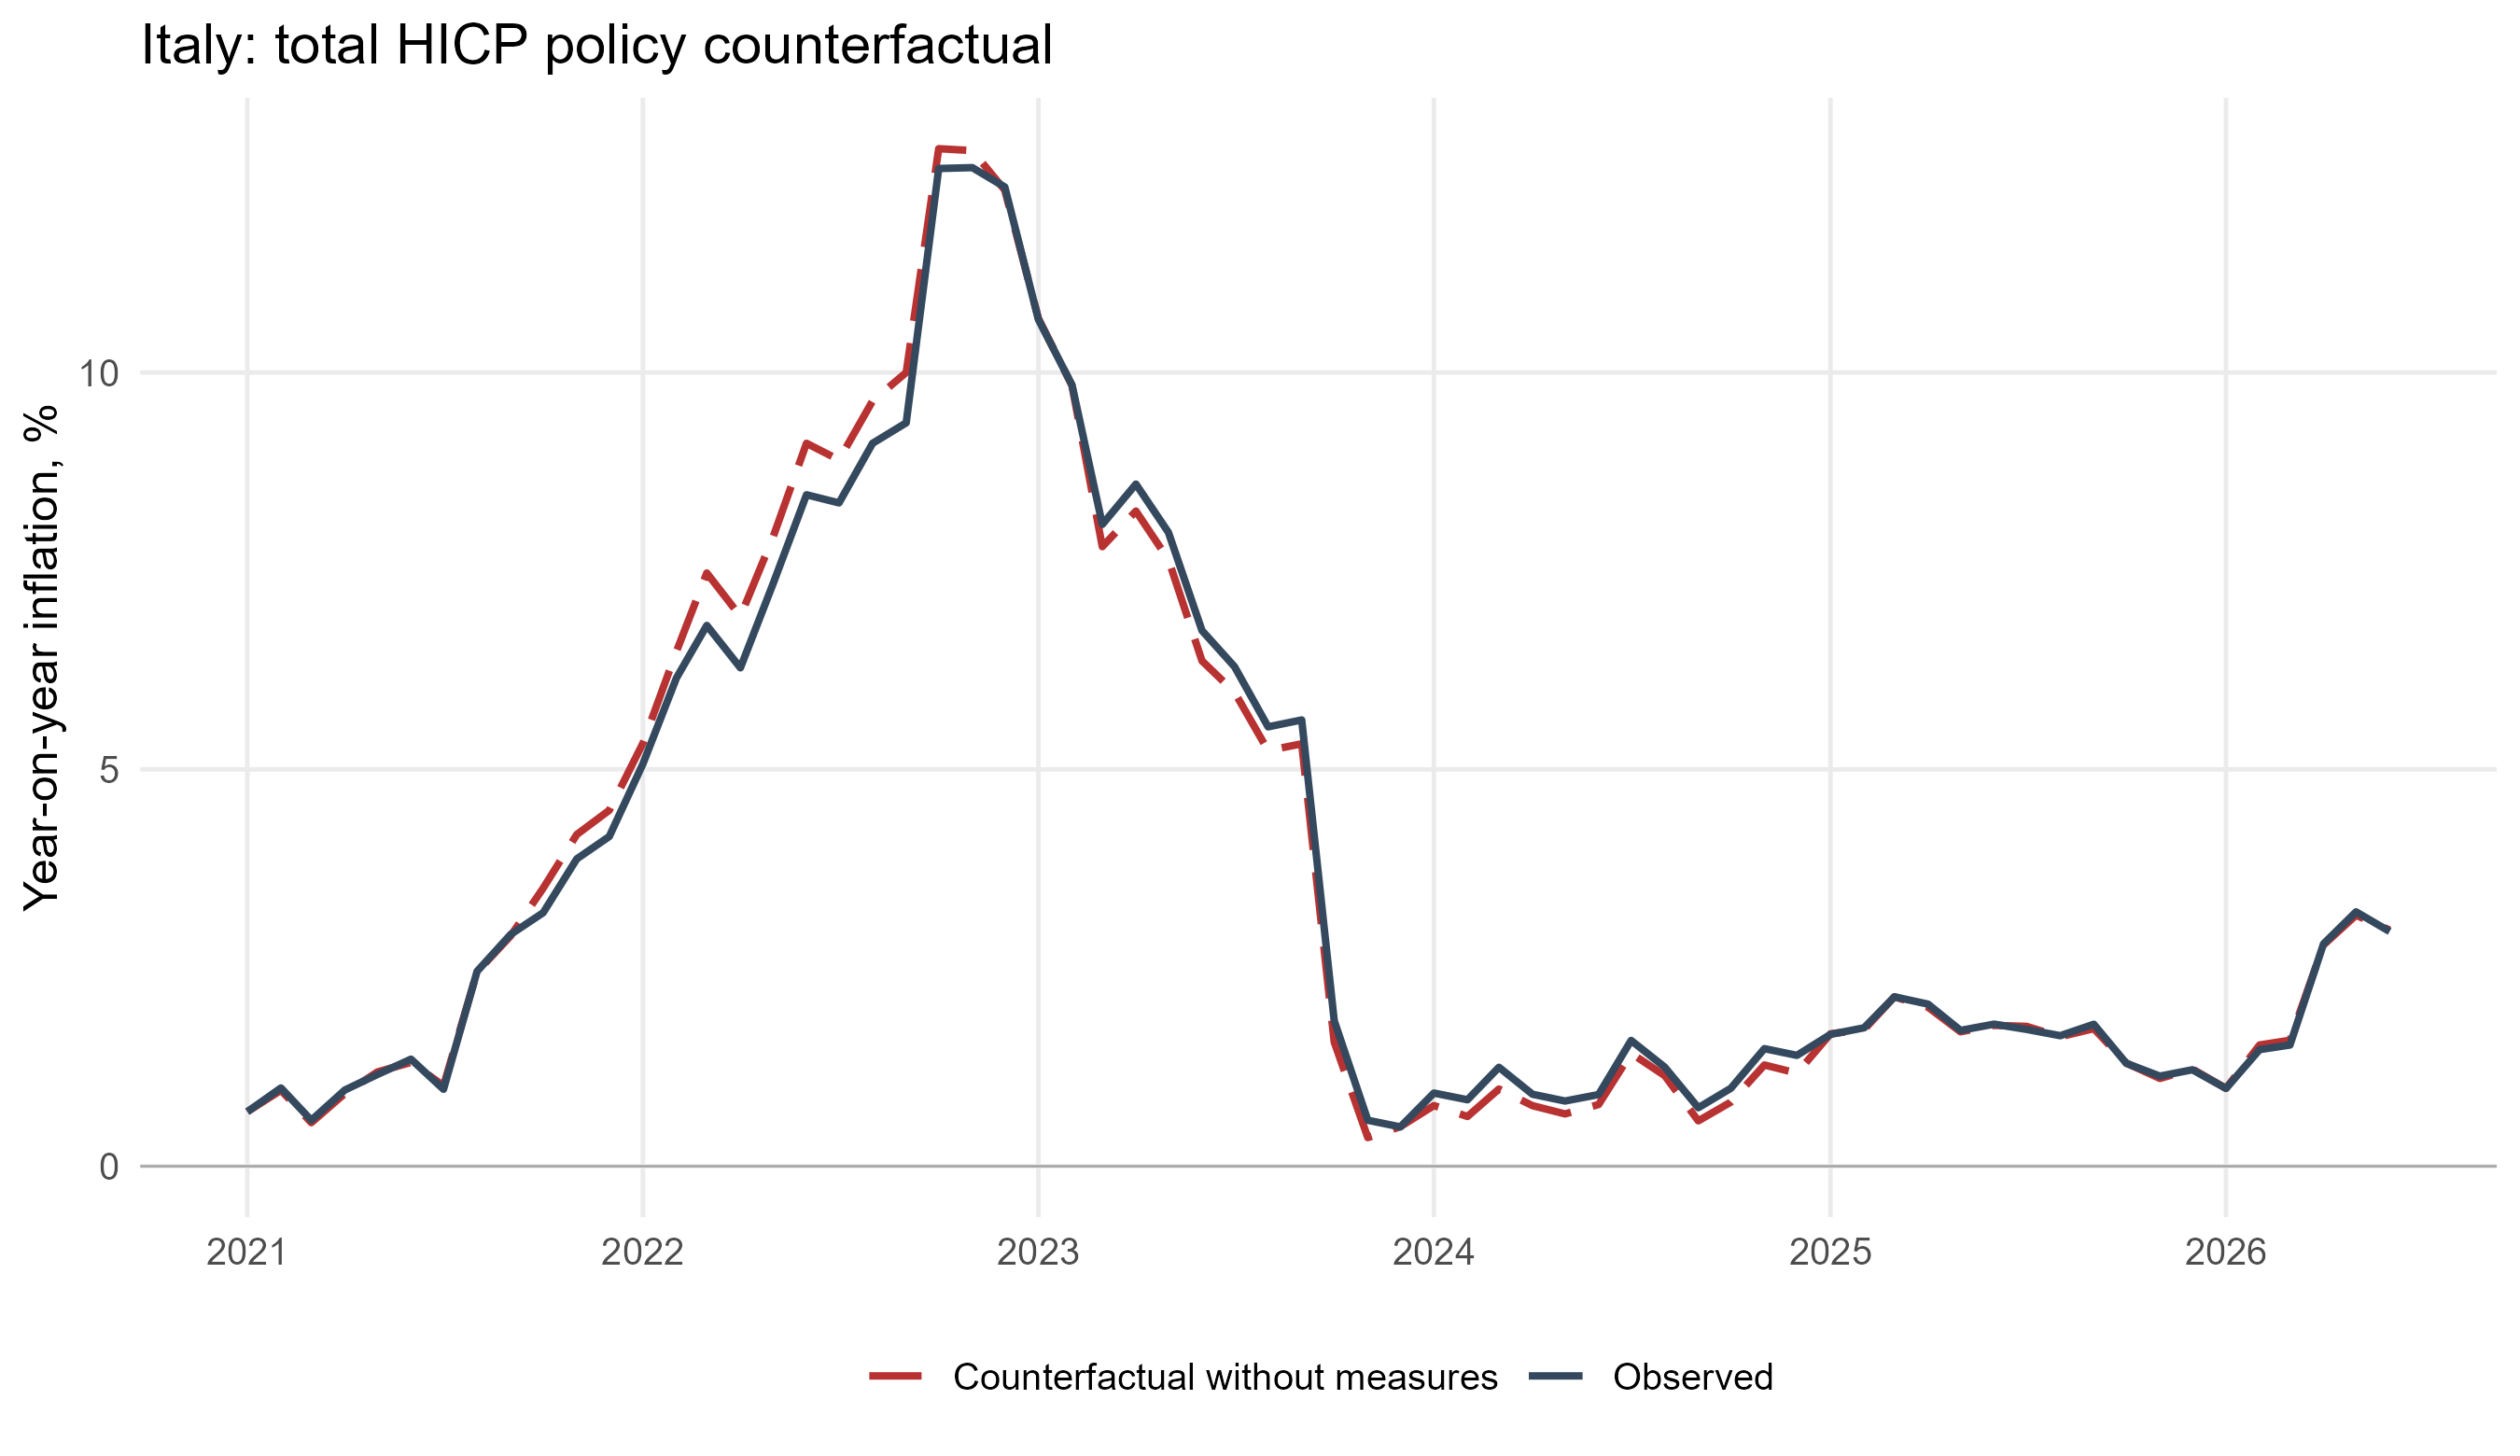
\includegraphics[width=0.86\textwidth,height=0.38\textheight,keepaspectratio]{fig/policy_total_cpi_counterfactual_inflation_IT_italy.png}
\caption{Italy: observed and counterfactual inflation}
\end{figure}

\subsection{Lithuania}
\begin{figure}[H]
\centering
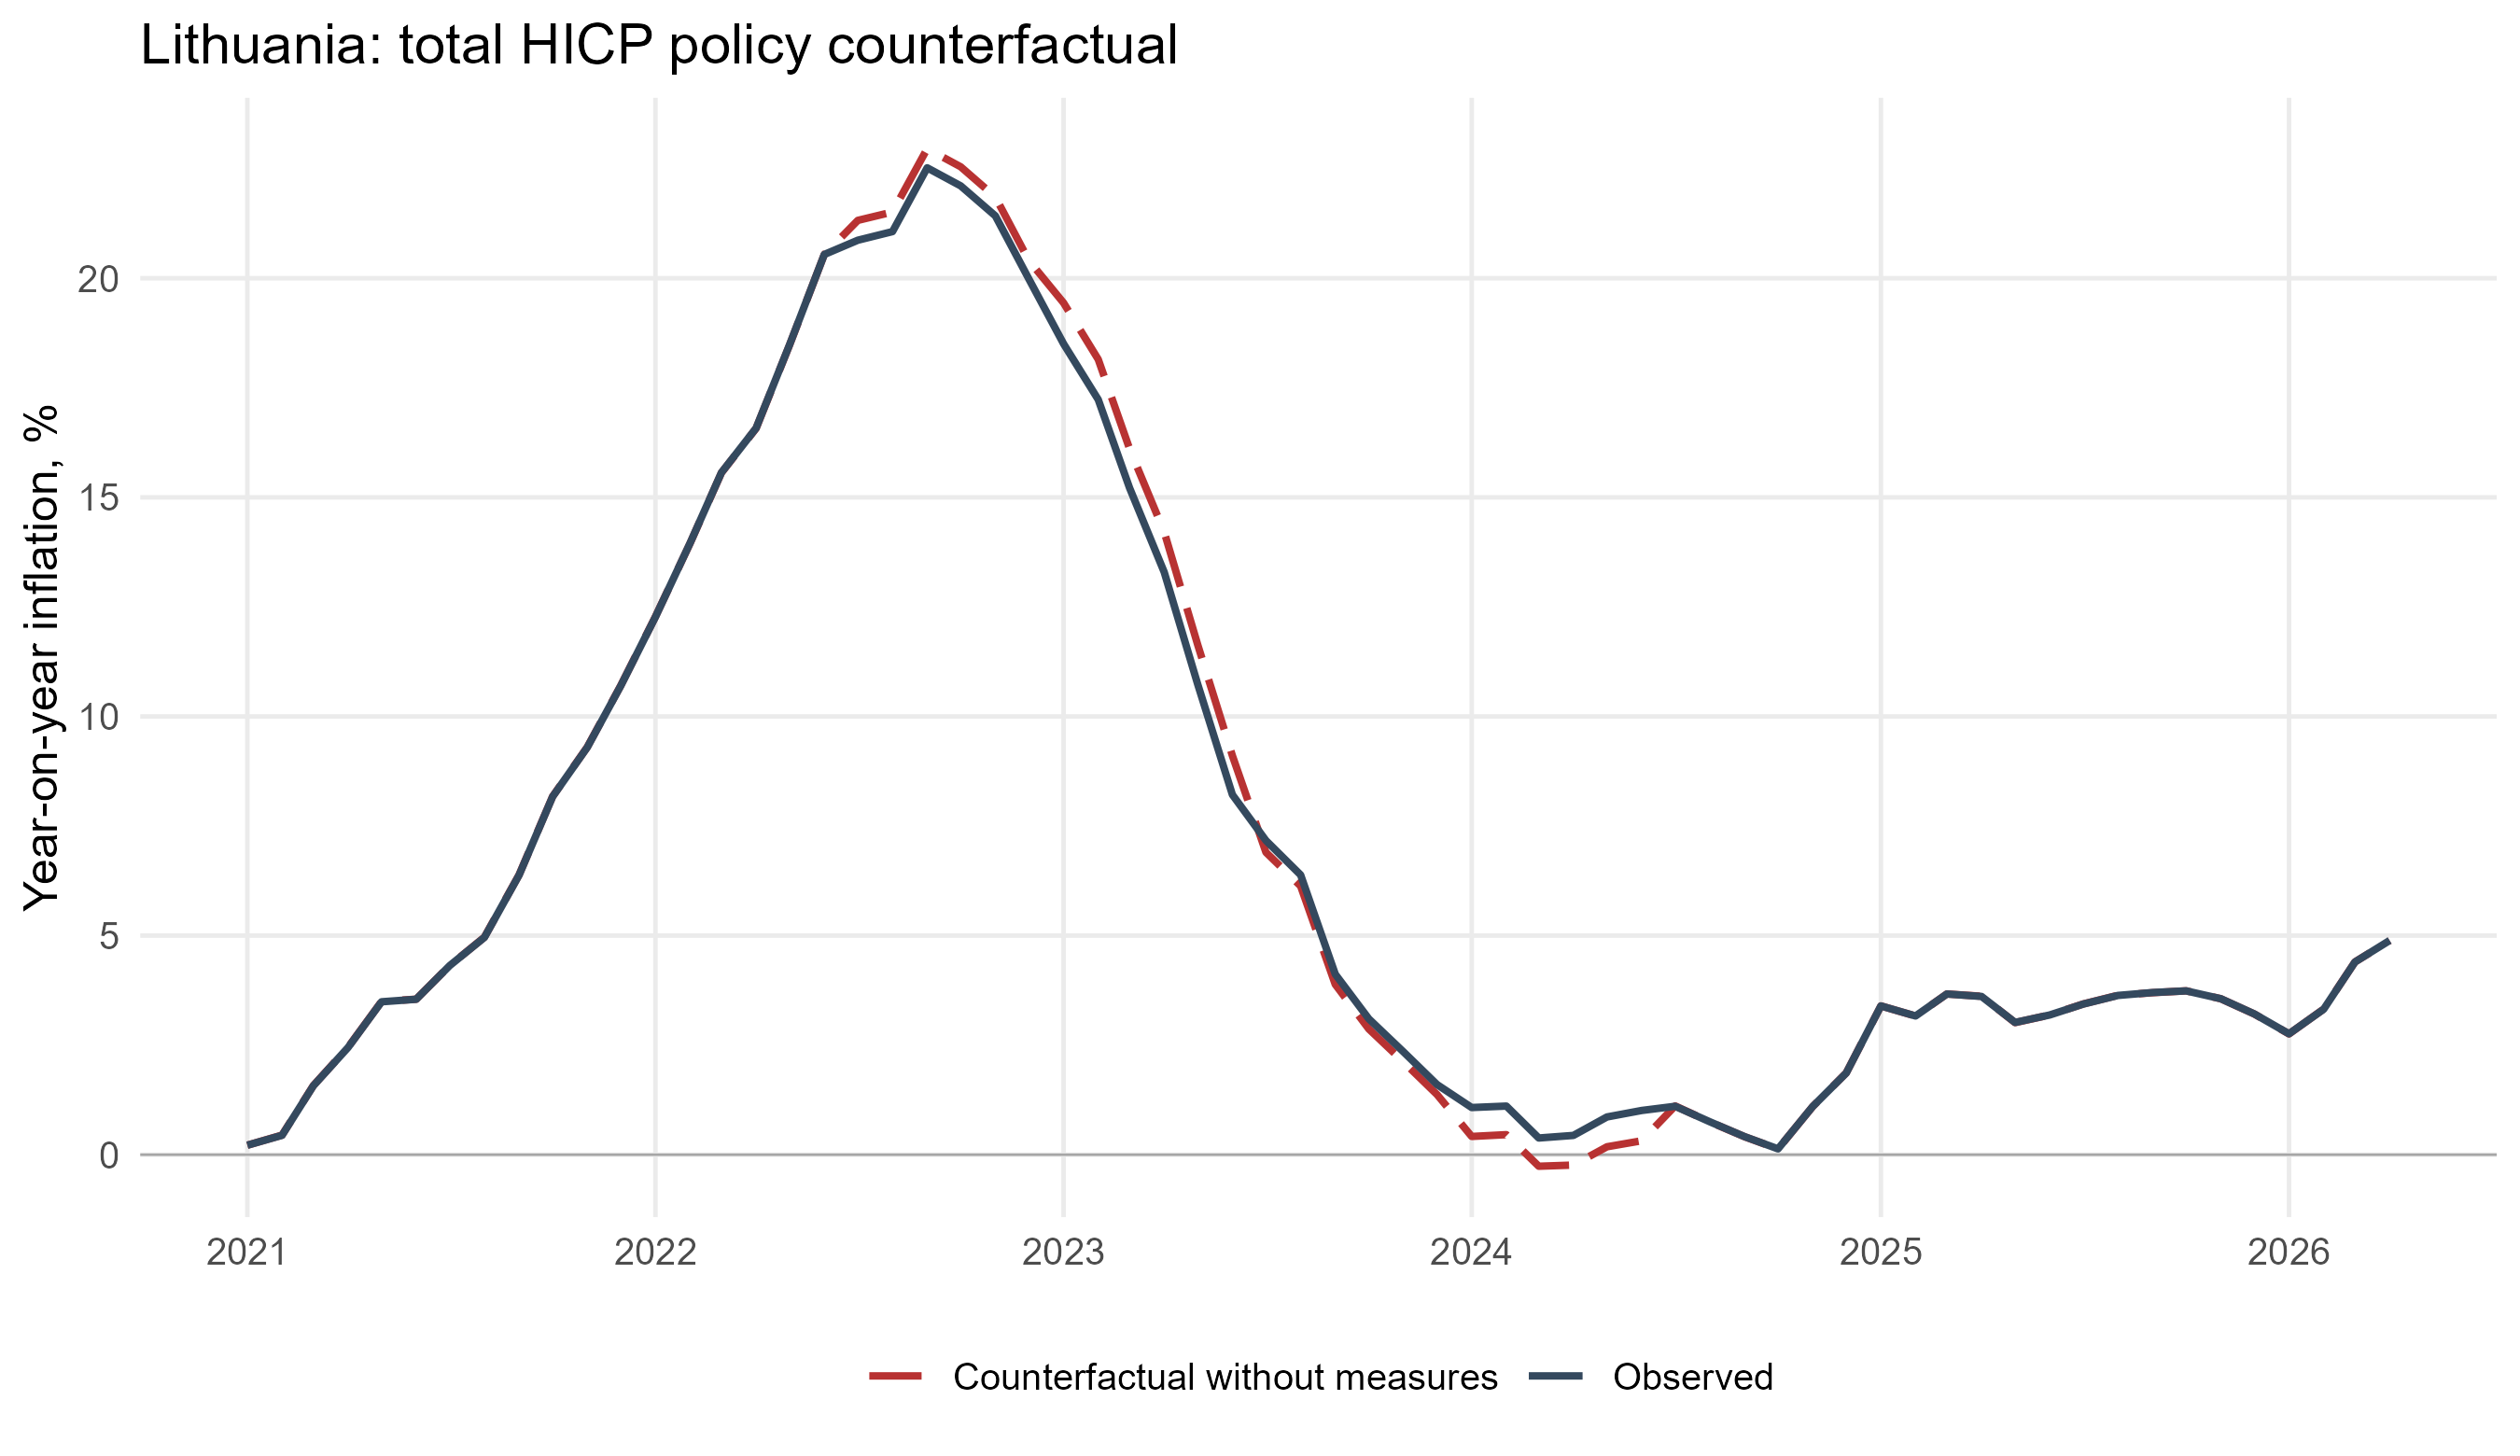
\includegraphics[width=0.86\textwidth,height=0.38\textheight,keepaspectratio]{fig/policy_total_cpi_counterfactual_inflation_LT_lithuania.png}
\caption{Lithuania: observed and counterfactual inflation}
\end{figure}

\subsection{Netherlands}
\begin{figure}[H]
\centering
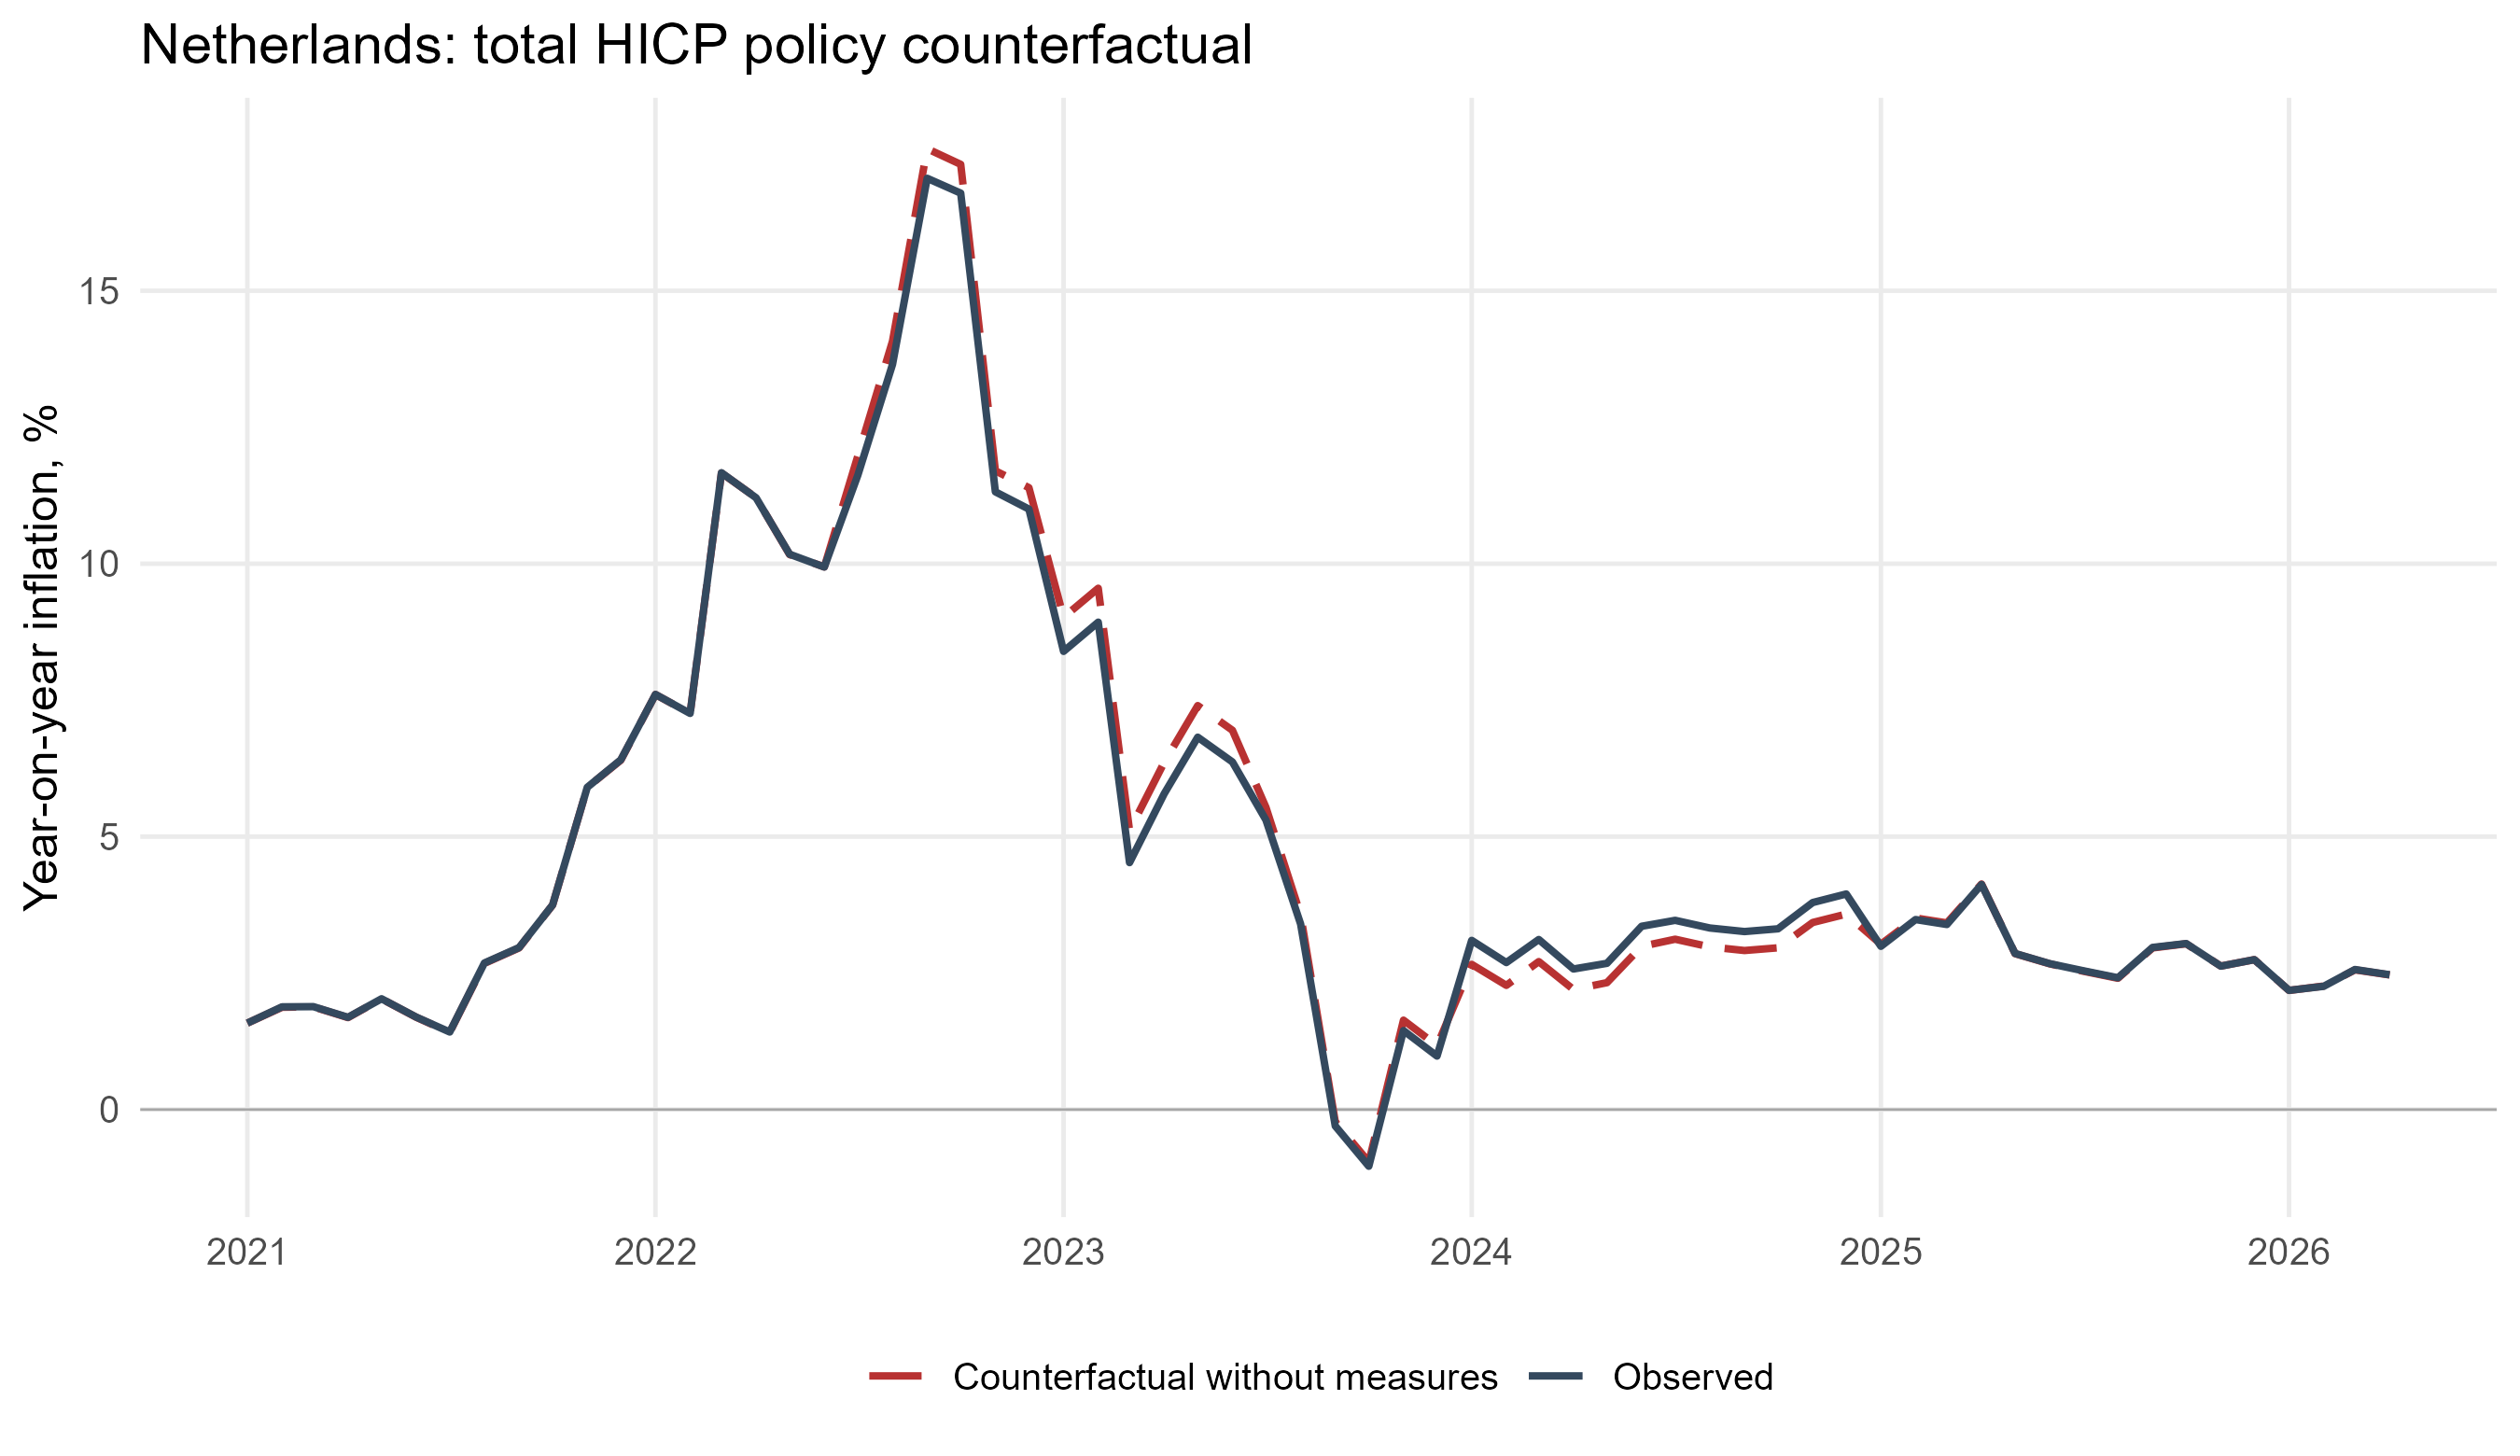
\includegraphics[width=0.86\textwidth,height=0.38\textheight,keepaspectratio]{fig/policy_total_cpi_counterfactual_inflation_NL_netherlands.png}
\caption{Netherlands: observed and counterfactual inflation}
\end{figure}

\subsection{Portugal}
\begin{figure}[H]
\centering
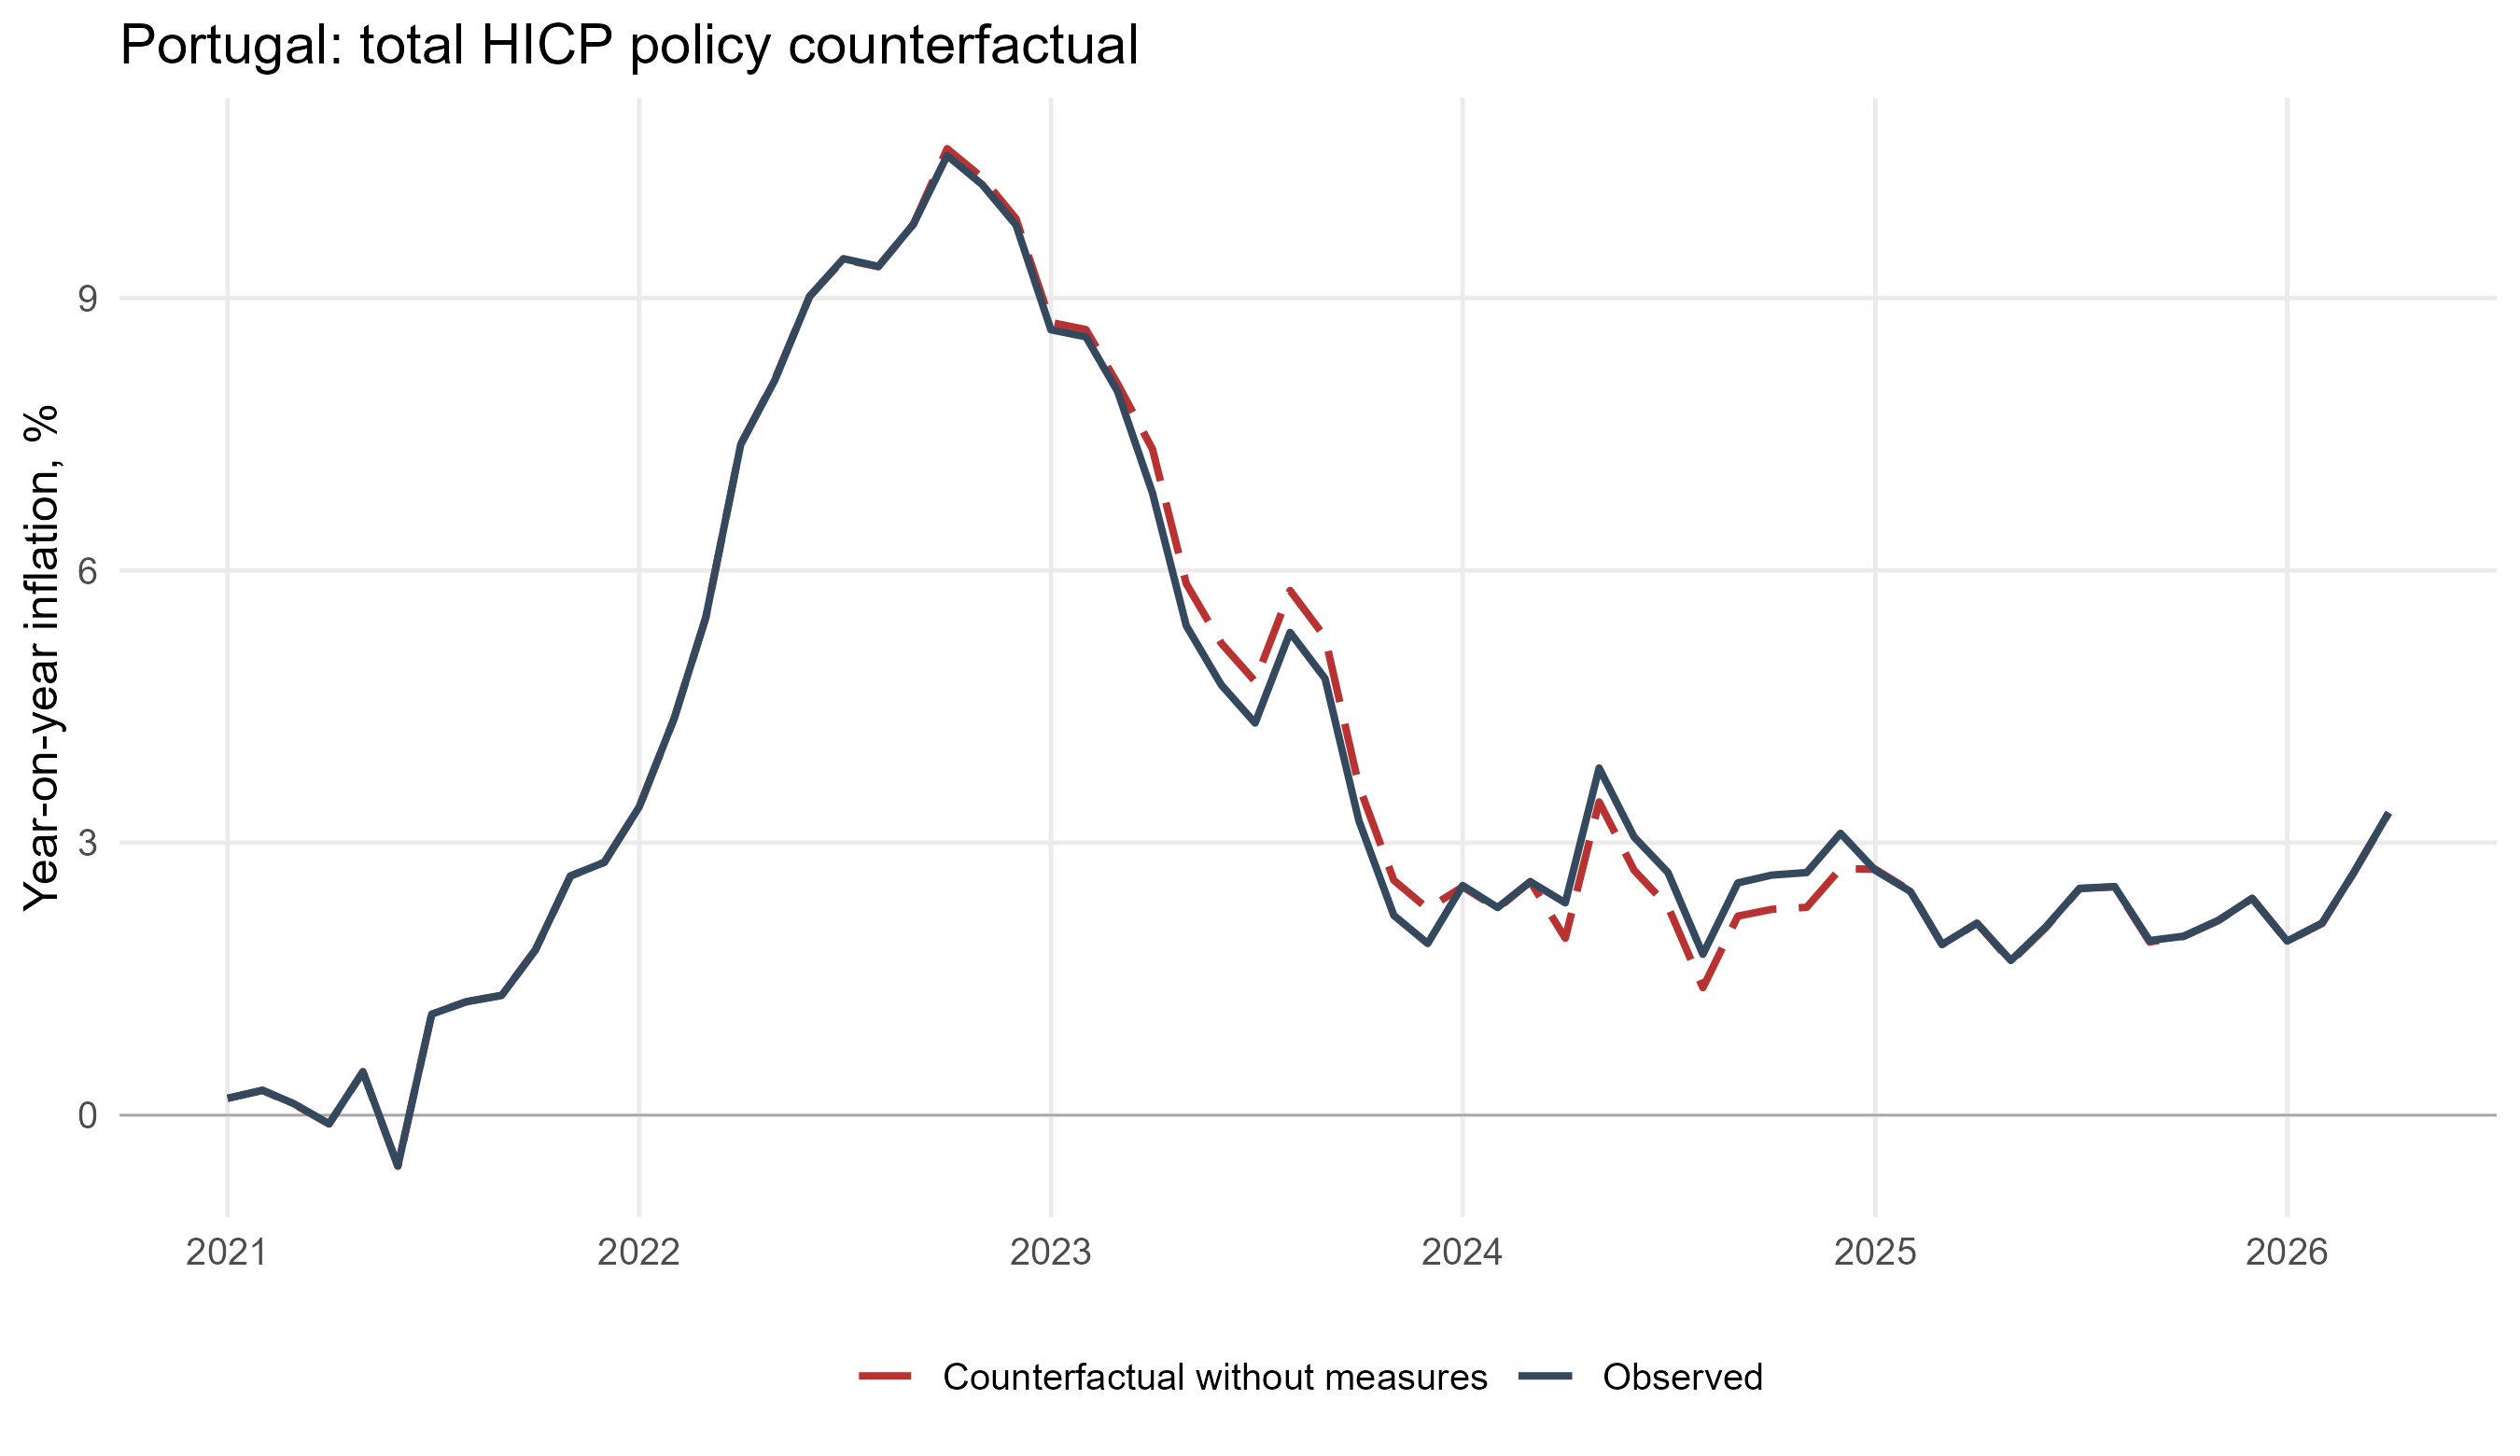
\includegraphics[width=0.86\textwidth,height=0.38\textheight,keepaspectratio]{fig/policy_total_cpi_counterfactual_inflation_PT_portugal.png}
\caption{Portugal: observed and counterfactual inflation}
\end{figure}

\subsection{Slovenia}
\begin{figure}[H]
\centering
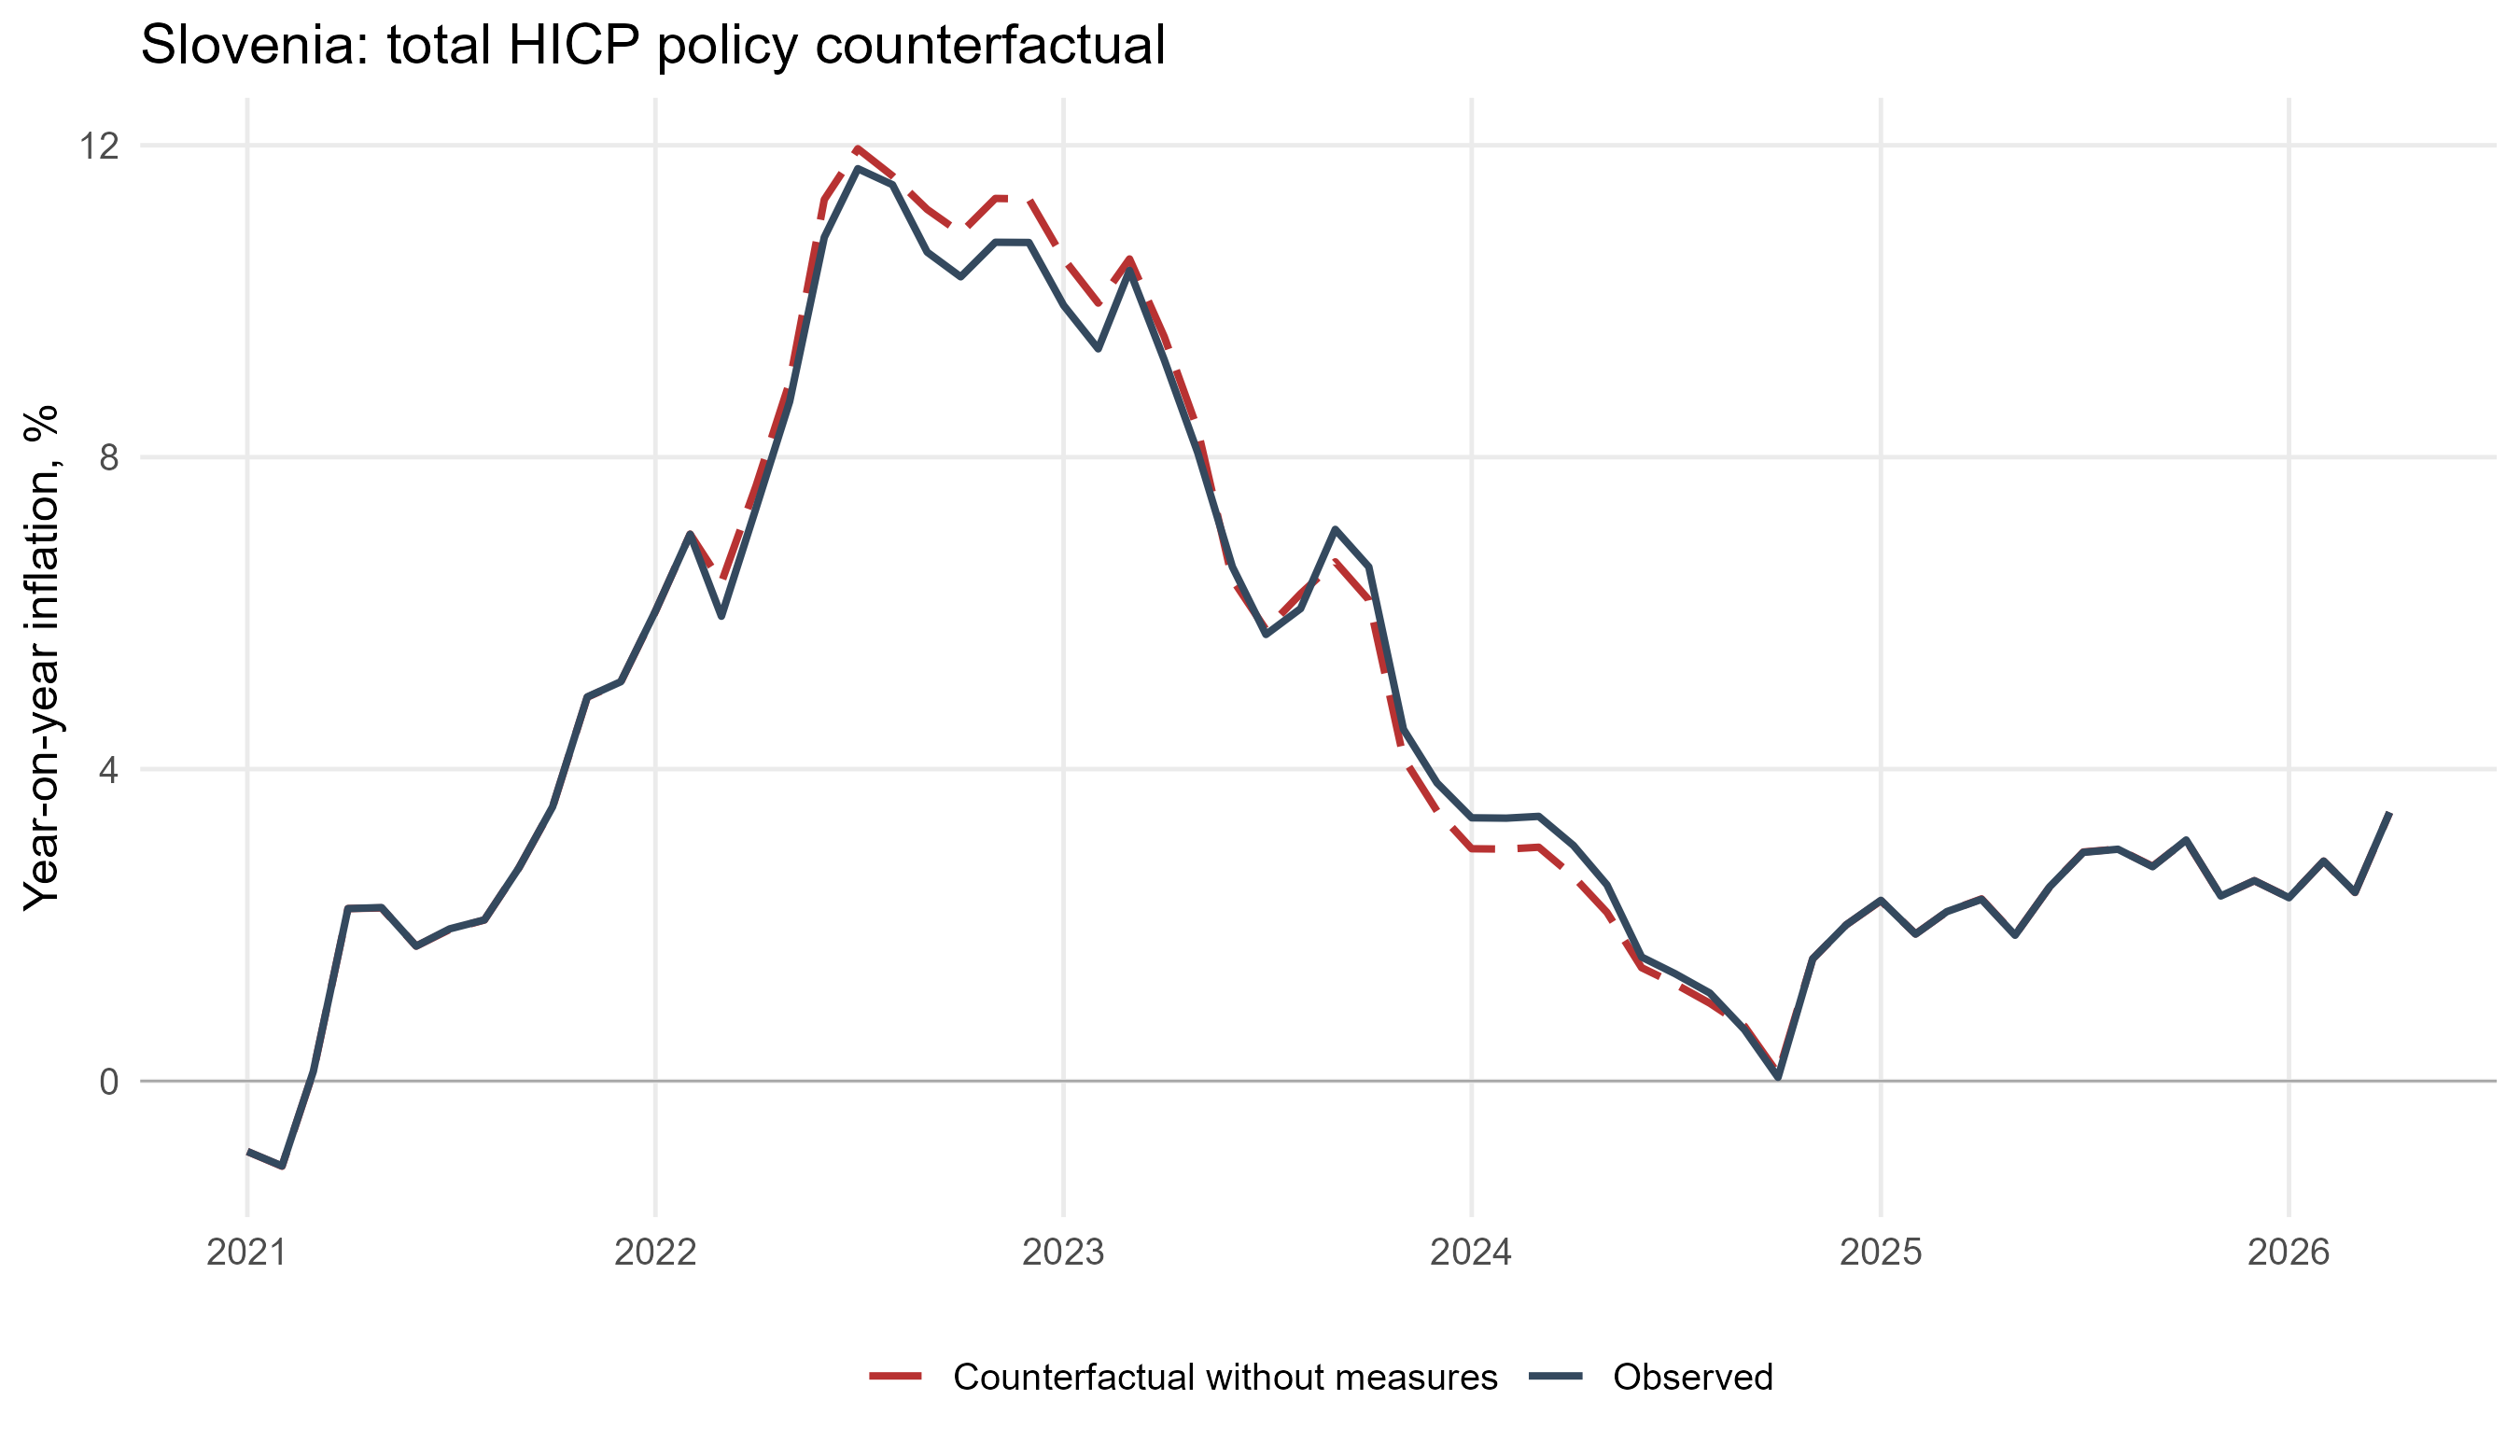
\includegraphics[width=0.86\textwidth,height=0.38\textheight,keepaspectratio]{fig/policy_total_cpi_counterfactual_inflation_SI_slovenia.png}
\caption{Slovenia: observed and counterfactual inflation}
\end{figure}

